\chapter{Algoritmus elhelyezése ROS-ban}
\label{sec:inros}

Ebben a fejezetben leírom, hogyan helyeztem el a tervezett algoritmust ROS-on (Robot Operating System-en) \cite{ros} belül. Kitérek az ROS fejlesztési elveire, illetve az algoritmus leírásában használt kifejezésekre, melyek szükségesek a megértésben. Bemutatom a tervezett csomagot, elemeit és működését. Használt kommunikációs csatornákat, rétegeket és a felhasznált modulokat, könyvtárakat. A fogalmak bemutatásához az ROS dokumentációját \cite{ros} használtam alapul.

\section{ROS bemutatása}
A ROS (Robot Operating System) könyvtárakat és eszközöket biztosít, amelyek segítenek a szoftverfejlesztőknek robotokon alkalmazások létrehozásában. Hardveres absztrakciót, eszközillesztőket, könyvtárakat, megjelenítőket, üzenettovábbítást, csomagkezelést és még sok mást eszközt biztosít egy környezetben. A ROS nyílt forráskódú, BSD licensz\footnote{BSD licensz: \url{https://www.freebsd.org/copyright/freebsd-license/}} alatt van licencelve.

A ROS egy meta-operációs rendszer, mely olyan szolgáltatásokat is nyújt, amelyek egy operációs rendszerben eleve be vannak építve, beleértve a hardveres absztrakciót, az alacsony szintű eszközvezérlést, az általánosan használt funkciók megvalósítását, a folyamatok közötti üzenettovábbítást és a csomagkezelést. Megkönnyíti csomagok létrehozását és futtatását több számítógépen, ehhez eszközöket és könyvtárakat biztosít.

ROS-ban létrehozott számítási gráffal (Computation Graph) modellezhető kommunikációs kapcsolatok hálózata és „peer-to-peer" megvalósítása. Többféle kommunikáció valósítható meg ROS-on belül, szinkron kommunikáció formájában „service”-eken keresztül vagy aszinkron „topic”-okon keresztül. Adatok tárolását „parameter server”-en biztosítja.
A ROS célja, hogy a megírt kód újrafelhasználható legyen különböző kutatásokban, fejlesztésekben. Folyamatok alá egy elosztott keretrendszert biztosít. „Node”-ok hozhatók létre, ezek olyan egységek, melyek képesek információkat küldeni, fogadni vagy feldolgozni és továbbítani. A „node”-ok ROS-on belül elkülönült rendszereket alkotnak, a változókat külön képesek kezelni, de egymással meg is tudják azokat osztani. Ennek a felépítésnek előnye, hogy komplex a folyamatokat, rendszereket könnyen átlátható részekre lehet szétbontani.

\section{ROS keretrendszer elvei} %TODO ITT TARTOK 23:18
A készítők minimális tárhely igényre és az írt kódok felhasználók közötti megosztásának megkönnyítésére törekedtek, mely segíti az integrálást különböző robotokra tervezett keretrendszerekkel. A ROS-t már integrálták az OpenRAVE-vel, az Orocos-szal és a Player-rel. Pythonn és C++ programozási nyelven van lehetőség csomagok fejlesztésére. Tesztelést megkönnyíti a „rostest”: beépített tesztrendszer, amely aszisztál tesztek írásában és lebonyolításában. A ROS alkalmas nagy futásidejű rendszerek és hosszú fejlesztési folyamatok kivitelezéséhez.

\section{ROS-ban használt fogalmak}
Három szintre különíthető el a ROS felépítése\footnote{ROS concepts: \url{http://wiki.ros.org/ROS/Concepts}}: fájlrendszer (Filesystem level), számítási gráf (Computation Graph) és a közösség (Community) által fejlesztett csomagok szintje. A fájlrendszer szintű fogalmak főként a lemezen, tárhelyen található ROS erőforrásokra vonatkoznak. A Computation Graph a „node”-ok kapcsolata, gráfelméleti értelmezésében „node”-ok alkotják a gráf csomópontjait. Ebben a fejezetben e két koncepciós szint fogalmait mutatom be a dolgozat érdemi részének megértése céljából.

\subsection{ROS fájlrendszer}
\subsubsection{Csomagok}
A csomagok jelentik a szoftverek ROS rendszerben való rendszerezésének fő egységeit. Egy csomag tartalmazhat ROS futásidejű folyamatokat („node”-okat), ROS-tól függő könyvtárat, adatkészleteket, konfigurációs fájlokat vagy bármi mást, ami hasznosan össze van szervezve futtatáshoz. A csomagok a ROS legmagasabb szervezettségi szintjei, a legkomplexebb egység, amit összeállíthat és kiadhat egy fejlesztő, egy csomag.

%\subsubsection{Meta-csomagok}
%A meta-csomagok speciális csomagok, amelyek egymáshoz kapcsolódó csomagokat tartalmaznak. A meta-csomagokat használhatók verziók közötti kompatibilis megoldásához.

\subsubsection{Package manifest}
A manifest-ek a csomagok főkönyvtárában található (A \verb|package.xml|) fájlok, melyek meta adatokat adnak a csomagokról, beleértve a fejlesztő nevét, a csomag verzióját, leírását, licencinformációit, függőségeit és egyéb meta információkat, például a használt „exportált” csomagokat. A \verb|package.xml| csomagjegyzékek REP-0127-es\footnote{REP-0127: \url{https://www.ros.org/reps/rep-0127.html}} szabvány szerint vannak definiálva.

\subsubsection{Repository}
Egy repository az ugyanazon ROS verzióra készült csomagok gyűjteménye, egy projekthez tartozó csomagok összesége. Egy robothoz tartozó „repository” tartalmazza a működéséhez szükséges telepített és használt csomagokat.

\subsubsection{Üzenet „message” leíró fájlok}
A \verb|.msg| kiterjesztésű fájlokban kell definiálni az üzenetek leírását, a kommunikáció adatszerkezetét. Csomagonként lehet definiálni különböző \verb|.msg| fájlokat, általánosan a \verb|package/srv/MyServiceType.srv| elérési útvonalon. Egy csomagban definiált üzenet másik csomagban is hivatkozható és használható lesz, fordítás és megfelelő függőségek megadása után.

\subsubsection{Szolgáltatás „service” leíró fájlok}
A \verb|.srv|” kiterjesztésű fájlokban leírt szolgáltatások határozzák meg a kérések („request”) és válaszok („response”) adatstruktúráit. Általános elérési útvonaluk: \verb|package/srv/MyServiceType.srv|. Az üzenetekkel egyező módon, egy csomagban definiált „service”-ek másik csomagban is hivatkozhatóak és használhatóak lesz.

%TODO új oldal?
\subsection{Computation Graph}
ROS folyamatok „peer-to-peer" hálózata, amelyek együtt dolgoznak fel adatokat. A hálózatot leíró folyamatok kommunikációs hálójának rendszerezési fogalma a fájlrendszer feletti architekturális szinten a „Computation Graph”. A következő pontokban a gráfot alkotó elemeket mutatom be.

\subsubsection{Node-ok}
A „node”-ok vagy csomópontok, olyan folyamatok, amelyek számítást, adatfeldolgozást végeznek. ROS moduláris felépítésének egységei. „Node”-okba szokás csoportosítani a különböző feladatokat, például egy „node” felelős a térképezésért, egy másik pedig a motorok vezérléséért. ROS-ban „node”-okat írhatunk C++ nyelven „roscpp”\footnote{roscpp: \url{http://wiki.ros.org/roscpp}} vagy Python nyelven a „rospy”\footnote{rospy: \url{http://wiki.ros.org/rospy}} könyvtárak („ROS client library”-k) felhasználásával.

\subsubsection{ROS Master}
Egy „nameservice”, tárolja a gráf „node”-jainak információit, segítségével találják meg egymást a „node”-ok és tudnak üzeneteket küldeni, szolgáltatásokat hívni. A „ROS Master" névadási és regisztrációs szolgáltatásokat nyújt a ROS rendszer minden „node”-ja számára. Nyomon követi a „topic”-ok „publisher”-eit és „subscriber”-eit és „service”-eket. A „Master" szerepe az, hogy lehetővé tegye az egyes ROS „node”-oknak egymás helyének meghatározását. Miután ezek a csomópontok megtalálták egymást, „peer-to-peer" kommunikációval közölhetnek adatokat egymással. A „Master" biztosítja a „parameter server"-t is.

\subsubsection{Parameter Server}
Lehetővé teszi kulcs és adat párok tárolását, a „Master" része. Innen elérhetőek a paraméterek a „node”-ok számára. Ilyen paraméterek lehetnek a robot fizikai dimenziói, mozgásra képes alkatrészek rotációja, elmozdulása, csatlakozó pontok és a robothoz kapcsolt szenzorok koordinátái.

\subsubsection{Üzenetek - „messages”}
A „node”-ok üzenetek küldésével kommunikálhatnak egymással. Egy üzenet egy adatstruktúra, amely adattípust és annak elnevezését tartalmazza. A szabványos primitív típusok (\verb|int, bool, float, string|) támogatottak, csakúgy, mint ezen primitív típusok tömbjei. Az üzenetek tetszőlegesen is tartalmazhatnak beágyazott, a felhasználó által primitív tagokból definiált struktúrákat és azok tömbjeit.

\subsubsection{Topic-ok}
A „topic”-ok vagy témák, az üzenetek továbbítására használt csatornák küldő-fogadó (subscriber-publisher) szemantikával. Egy „node” úgy küld üzenetet, hogy közzéteszi azt egy adott „topic”-on. A „topic” egy név, amely az üzenet tartalmának azonosítására szolgál. Egy bizonyos típusú adat iránt érdeklődő „node” feliratkozhat a megfelelő „topic”-ra. Az adott „topic”-on minden publikált adat után meghívódik a feliratkozott „node”-ban egy „callback” függvény, amelyben feldolgozhatjuk a kapott adatot. Egy „topic”-nak több adója és feliratkozója lehet egyidejűleg, és egyetlen „node” több „topic”-on is közzétehet és feliratkozhat rá. Általában az adók és a feliratkozók nincsenek tudatában egymás létezésének. Az információtermelést leválasztják annak fogyasztásáról. Egy „topic”-ot egy virtuális üzenetbusznak tekinthetünk. Minden busznak van neve, és bárki csatlakozhat a buszhoz üzenetek küldése vagy fogadása céljából, amennyiben az adatcsomag típusa megfelelő.

\subsubsection{Szolgáltatások - „services”}
A „subscriber-publisher” kommunikációs paradigma „many-to-many" azaz többen publikálhatnak a csatornára és többen is elérhetik az adatot, ezzel szemben a szolgáltatások két „node” között teremtenek kommunikációs csatornát. A modell: kérés-válasz (request-reply), azaz egy szerver „node” bizonyos név alatt egy szolgáltatást biztosít, amit egy másik „node”-on belül meg tudunk hívni. A hívás következtében a szerverként működő „node” meghív egy függvényt, így tekinthető távoli eljáráshívásnak. A hívó „node” megvárja a választ, ezzel megakasztva belső működését.

\section{ROS verzió}
ROS-ból léteznek disztribúciók, amik különböző fő verziókat jelentenek, ezekbe csoportosítva a ROS csomagokat. A disztribúciók célja, hogy lehetővé tegyék a fejlesztőknek, hogy egy stabil kódbázissal dolgozzanak mindaddig, amíg készen nem állnak az új verzióra való átállásra. Disztribúciók kiadása után korlátolt mértékben hibajavítások még fejlesztésre kerülnek hozzájuk, de jellemzően semmi olyan frissítést nem adnak ki a ROS fejlesztői, ami eltörné a kommunikációt azonos disztribúcióra írt csomagok között. A disztibúciók kiadása a Linux Ubuntu operációs rendszer fő verzióinak kiadását követi.

A Biscee roboton jelenleg futó csomagok nagy része ROS Melodic\footnote{ROS Melodic Morenia: \url{http://wiki.ros.org/melodic}} verzió alatt lett fejlesztve. Mivel csak a Python 2-es verziója használható csomagok fejlesztésére ez a verzió alatt, ezért kénytelen voltam ROS Noetic-et\footnote{ROS Noetic Ninjemys: \url{http://wiki.ros.org/noetic}} használni, ami már támogatja a Python 3-at, ami elengedhetetlen az OpenCV használatához. A különböző verziók közötti átjárásra már vannak létező megoldások, ezért nem limitálja az algoritmus használatát a roboton.

\section{ROS node-ok és kommunikációjuk}
A „node”-ok A ROS számítást végző egységei. Kombinációjuk gráfot alkot (Computation Graph) és „topic”-okon vagy „service”-eken keresztül kommunikálnak egymással. A cél, hogy egy „node” egy kiosztott feladatot lásson el, elszeparálva ROS-on belül a robothoz szükséges folyamatokat kisebb egységekre. Ennek előnye, hogy segíti a hibakeresést, egy-egy feladat felülvizsgálatához vagy lecseréléséhez elég az ezt specifikusan ellátó „node” vizsgálata, ismerete. Az esetleges hibák izolálva vannak „node”-okon belül így egy „node” leállása nem hat ki a robot teljes működésére, nem gátolja a többi „node” operációját. Megosztott feladatok miatt az egy helyre leírt kód mennyisége is csökken, ami átláthatóbbá teszi fejlesztői oldalról. Nem jelent problémát a különböző nyelven írt „node”-ok közötti kommunikáció sem, a ROS által biztosított komminkációs módok képesek áthidalni. Például egy „node” kezeli a lézeres távolság mérést, egy másik a motorok irányítását, külön „node”-ban implementálhatóak csak a lokalizációhoz tartozó feladatok és így tovább. A mintát követve, könnyen bővíthető és fejleszthető egy robot funkciókészlete.
Minden „node” rendelkezik egy névvel, ami egyedileg azonosítja a gráfban. ROS-ban „node”-okon belül egy programozási nyelv használható (Python vagy C++), melyekhez két könyvtár áll a fejlesztők rendelkezésére: „rosccp" és „rospy". Mivel a csomagot Python nyelven fejlesztettem, ezért a következő két szakaszban (\refstruc{sec:ros_sp1} és \refstruc{sec:ros_s2}) a „rospy" könyvtár által biztosított ROS architektúrába illeszkedő kommunikációs módokról írok.

\subsection{Subscriber-publisher modell}
\label{sec:ros_sp1}
% http://wiki.ros.org/rospy/Overview/Publishers%20and%20Subscribers
Aszinkron kommunikációs forma, röviden „Pub/Sub" minta, amit a szerver nélküli vagy mikroszolgáltatás architektúrákban használnak. Két elemből áll: egy küldő / „publisher” és egy fogadó / „subscriber”. A publisher elküldi az üzenetet, a subscriber fogadja. A modell két előnye, hogy segíti a kommunikációban résztvevő egységek független működését és használható eseményvezérelt programozásra. Ahogyan a \refstruc{fig:pubsub} is szemlélteti, a publisher-ek aszinkron módon küldhetnek üzenetet a csatornára, ami a megérkezésüknek megfelelő sorrendben a subscriber-ek részére elérhető. Az összes subscriber, ami ugyanarra a „topic”-ra van feliratkozva látja az összes publikált üzenetet. Az üzenet eljuttatása azonnal megtörténik, amint felkerült a „topic”-ra, ez különbözteti meg a hagyományos üzenetközvetítési modellektől, ahol a felhasználónak vagy szolgáltatásnak kell lekérnie az üzenetet. A „Pub/Sub" elgondolás elszigeteli a csatorna két oldalán levő „publisher"-eket a „subscriber"-ektől, azaz nem tudnak egymás létezéséről. Javítja ezzel az alkalmazás biztonságát. Aszinkronitása segíti a nagy forgalom melletti folyamatos működést. Az egységek (ROS esetében „node”-ok) közötti „Pub/Sub" modellben az üzeneteket egy „buffer”-be gyűjti, és a „buffer”-t minden „subscriber" kimenetére eljuttatja. Megadható a „buffer” mérete, vagyis hány üzenet eltárolására legyen alkalmas. Ennek megválasztása függ a használat céljától. Ha egy üzenetet meghatározott frekvencián küldünk, akkor célszerű akkora „buffer” méretet választani, ami a frekvenciához jól társul. Ha változó időközönként küldünk egy vagy több üzenetet célszerű nagyméretű „buffer”-t megadni. A „topic”-on közölt üzenetek adatmodelljét \verb|.msg| fájlokban lehet megadni, amiket aztán lefordít „roscpp"-ben és „rospy"-ban elérhető osztályokra \cite{pubsub1}\cite{pubsub2}.
\begin{figure}[!ht]
    \centering
    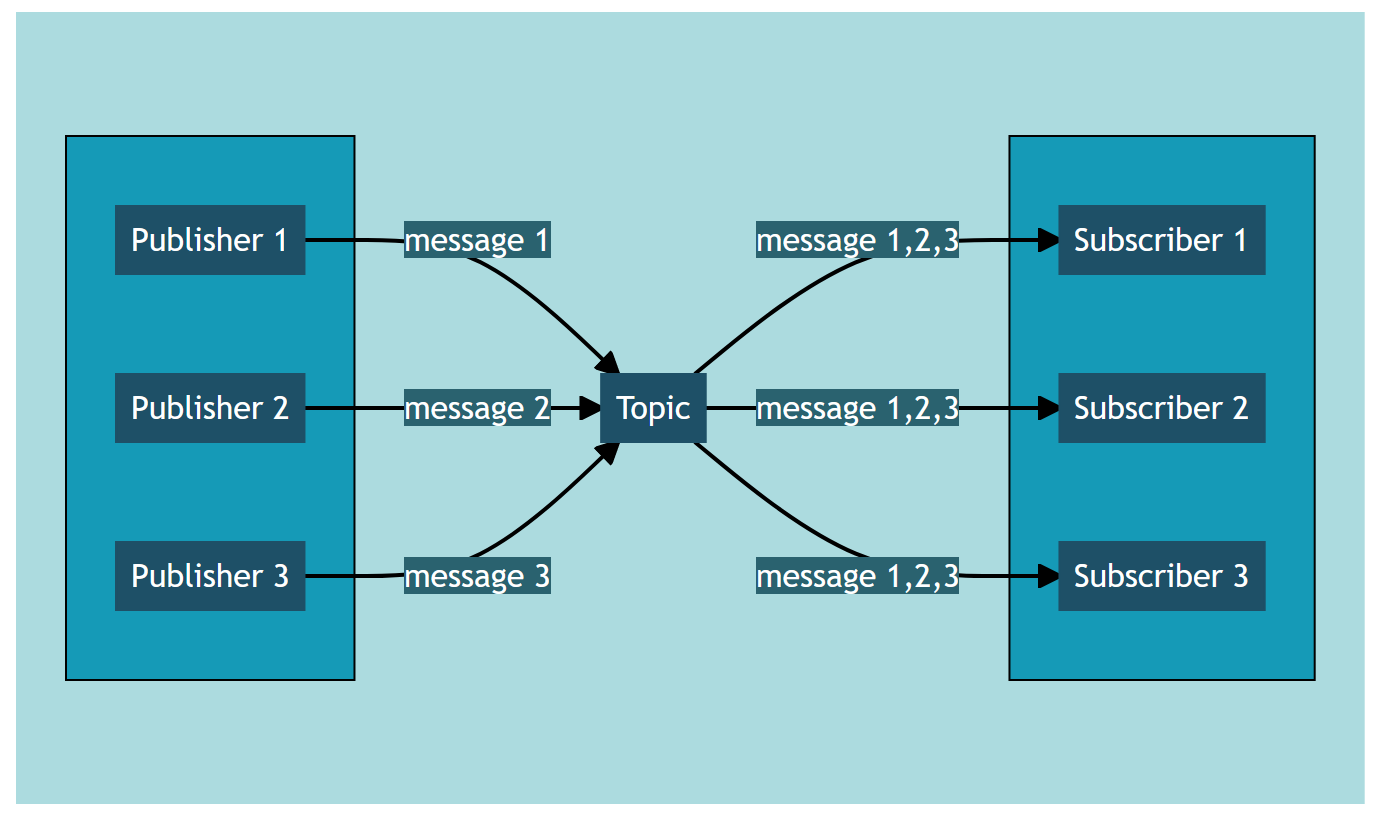
\includegraphics[width=150mm, keepaspectratio]{02_mermaid/mermaid02_pubsub.png}
    \caption{Publisher-subscriber modell.}
    \label{fig:pubsub}
\end{figure}
 \clearpage
\subsection{Service-request modell}
\label{sec:ros_s2}
% TODO forrás: http://wiki.ros.org/ROS/Tutorials/WritingServiceClient%28python%29
% https://learn.microsoft.com/en-us/azure/architecture/patterns/async-\verb|”request”|-reply
A szolgáltatások azaz „service"-ek egy másik mód a gráf „node”-jainak (csomópontjainak) kommunikációjára. A „service"-ek hívás-válasz (call-and-response) modellen alapulnak. Különbség a „topic”-okon való kommunikációval ellentétben, hogy csak akkor történik adatátadás, amikor egy kliens kifejezetten meghívja. Típusuk leírását \verb|.srv|” fájlban tehetjük meg, ami az üzenetek mintájára lefordul és utána hivatkozható lesz. Ugyanakkor az üzenetekhez képest két részből állnak: egy kérésből (request) és egy válaszból (response). A szolgáltatások meghívása szinkron történik. A kliens elindítja a „request”-et a szerver felé, mire a szerverben egy megadott „callback” függvény fut le. A futásidejétől függetlenül a kliens addig vár, amíg nem kapott valamilyen visszatérési értéket, amit a „response” tartalmaz. Amiben különbözik a „Pub/Sub” modelltől, hogy szinkron, azaz amíg a kliens a hívásra vár blokkolja a program futását. Célszerű olyan esetekben alkalmazni, amikor fontos információra vagy adatra van szükségünk. Ha a szolgáltatás meghívása után fel szeretnénk dolgozni az információt, vagy használni szeretnénk akkor előnyös, hogy megakasztja a futást a „response” beérkezéséig, s amint megérkezett az adat engedi, hogy fusson tovább a kód.
\begin{figure}[!ht]
    \centering
    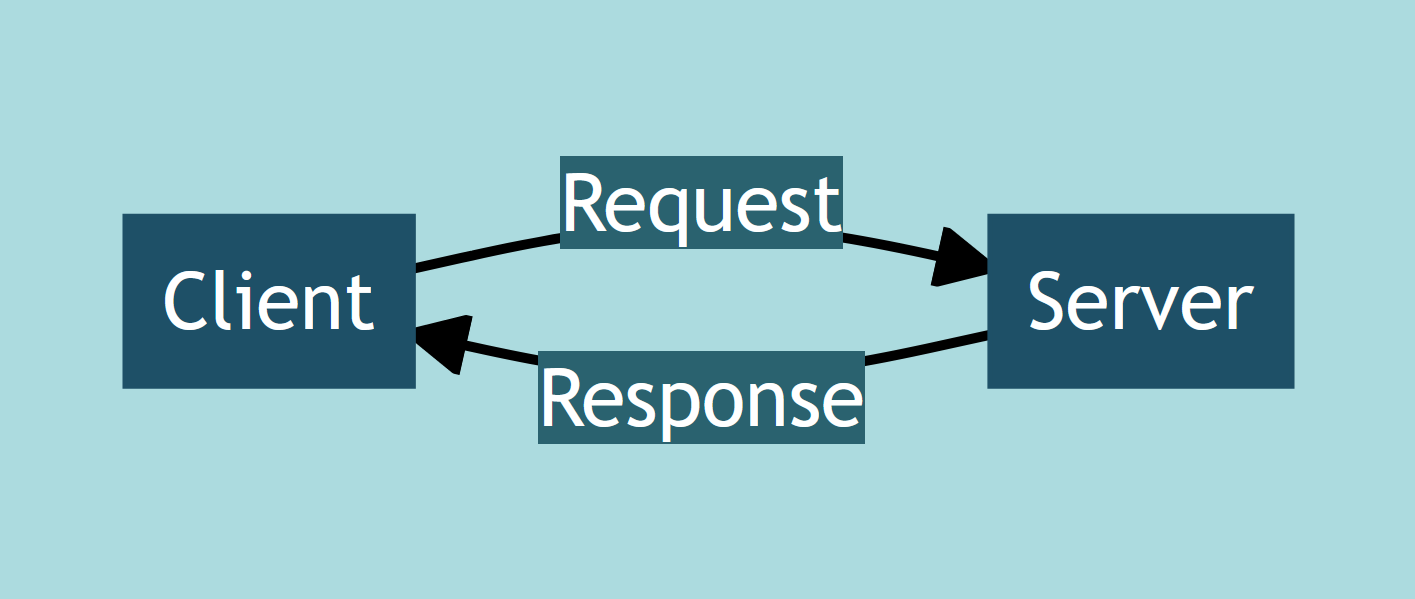
\includegraphics[width=100mm, keepaspectratio]{02_mermaid/mermaid03_service.png}
    \caption{Service-request modell.}
    \label{fig:service}
\end{figure}


\clearpage
\section{Tervezett csomag}
Ebben a fejezetben egy áttekintést biztosítok, milyen elemek alkotják az általam létrehozott csomagot. Leírom a ROS mellett használt fontos modulok működését, „node”-ok be- és kimeneteit alkotó „subscriber”-ek és „publisher”-ek és a bennük létrehozott változók, illetve függvények, melyek működésük megértésének szempontjából fontosak.

\subsection{Elhelyezés ROS-on belül}
ROS keretrendszer alapelveibe illeszkedően egy csomagot hoztam létre, ennek előnye, hogy bármilyen roboton, melyen ROS fut könnyen telepíthető. A csomag három „node”-ból áll. A külön „node”-ok létrehozása segíti a különböző folyamatok csoportosítását és az erőforrások felhasználásának ütemezését. A „node”-ok párhuzamosan futnak egymás mellett és „topic”-okon, illetve „service”-eken keresztül kommunikálnak egymással. A három „node” az alábbi ábrán látható (\refstruc{fig:fullmin}). A kamera képének elérésére készített „node” az OpenCV Python nyelvre készített csomagját\footnote{opencv-python: \url{https://pypi.org/project/opencv-python/}} használja. Az arcfelismerés fő folyamatára „Face recognition node” szolgál. Hozzá kapcsolódva egy külön \verb|ImageProcessor| osztályba szerveztem ki a kép feldolgozásával kapcsolatos feladatokat, mint az arcok észlelése és a felismert arcok megjelölése. A „Face database node” a \verb|DatabaseManager| osztályt használva kezeli és tárolja az adatokat. Az utolsó két „node” közösen támaszkodik a \verb|DataInterface| osztályra, az adattípusok közötti fordítások, átalakítások elvégzésében.

\begin{figure}[!ht]
    \centering
    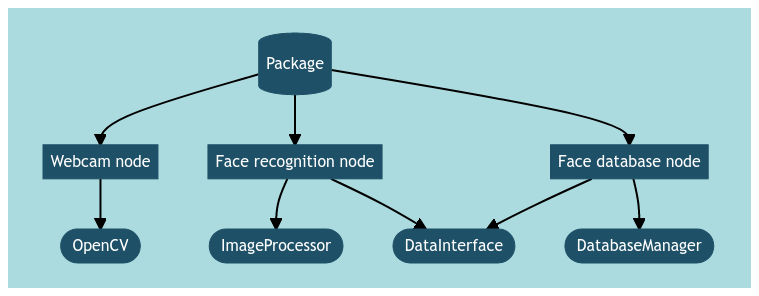
\includegraphics[width=150mm, keepaspectratio]{02_mermaid/mermaid01_minimal.png}
    \caption{Csomag belső kommunikációs csatornái.}
    \label{fig:fullmin}
\end{figure}

\clearpage
\subsection{Felépítés}
A három „node”-ot a csomag \verb|scripts| mappájában helyeztem el, alkalmazkodva a ROS-ban általánosan használt fájlrendszer kialakításhoz. Ezeket a „node”-okat: \verb|image_publisher.py|,  \verb|face_recognition_core.py| és \verb|face_database.py| fájlokban implementáltam. A ROS kétféle könyvtárat biztosít: „rospy” és „roscpp”, Python és C++ nyelvekhez. A fájlnevek kiterjesztéséből (.py) is látható, hogy python nyelven fejlesztettem. A választásom fő indoka, hogy ezen a nyelven van a legtöbb programozói tapasztalatom. További indoklás, hogy a Biscee roboton eddig alkalmazott csomagok nagy része is ezen a nyelven íródott, így fontos, hogy architekturálisan illeszkedjen ebbe a környezetbe, megkönnyítve a többi felhasználó és fejlesztő munkáját. Továbbá a használt „face-recognition" könyvtár is python nyelvben készült, ezért egyértelmű volt a választás.
\begin{figure}[!ht]
    \centering
    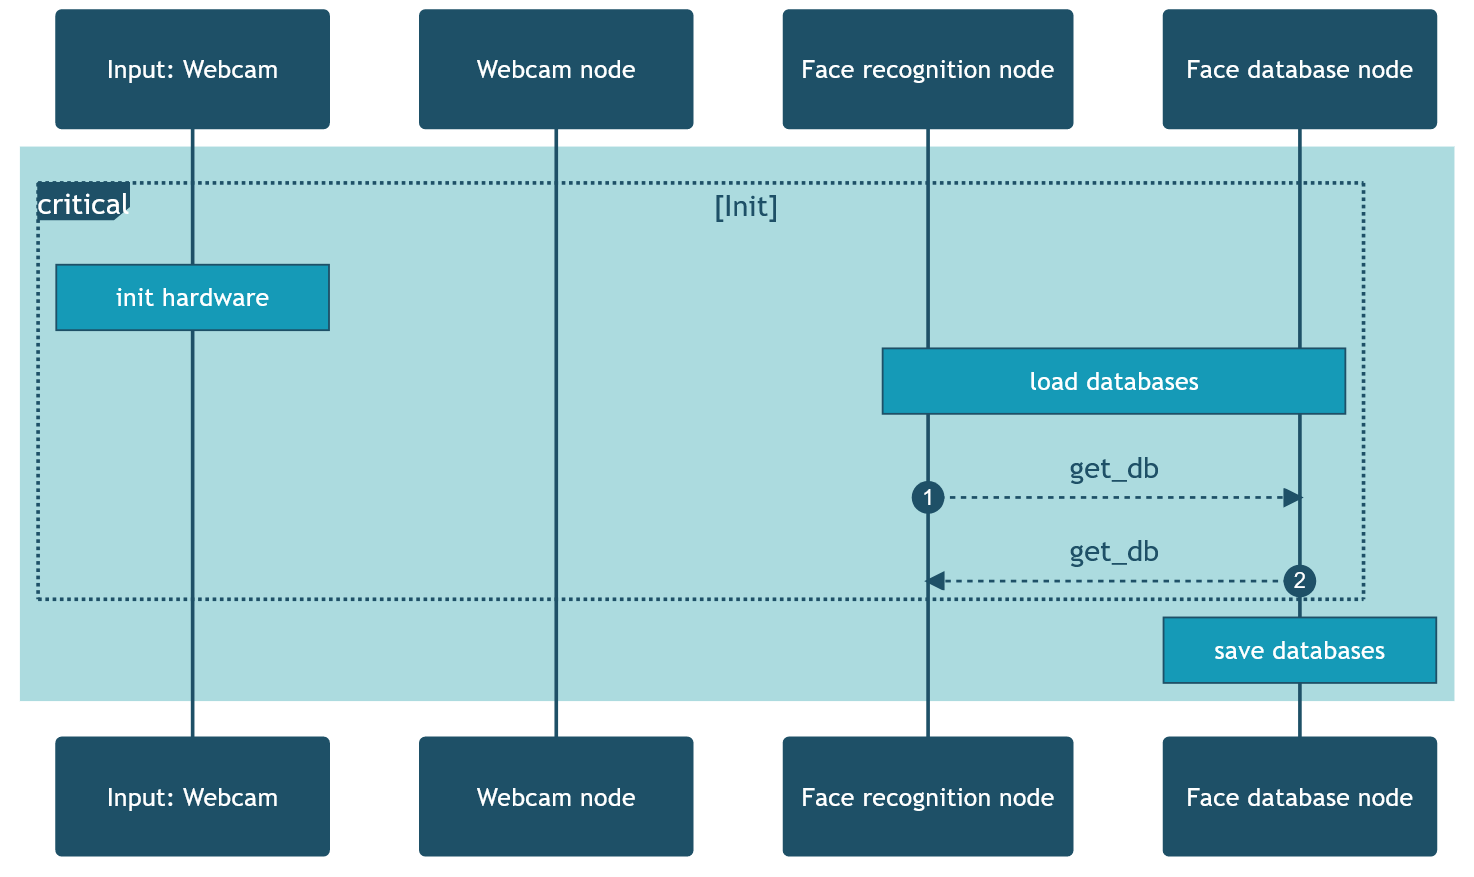
\includegraphics[width=155mm, keepaspectratio]{02_mermaid/full_init2.png}
    \caption{Csomag belső kommunikációs csatornái inicializáláskor.}
    \label{fig:fullcomm1}
\end{figure}
%TODO: részletes leírás a képről

A kommunikációs csatornák ábrázolása a „node”-ok, ki- és bemenetek között: inicializálás közben (\refstruc{fig:fullcomm1}) és működés közben (\refstruc{fig:fullcomm}). Működés közben használt „topic”-okat folytonos vonallal, a „service"-eket szaggatott vonallal ábrázoltam. Az inicializálás és működés közbeni kommunikációt a \refstruc{sec:modules}ban taglalom „node”-okra bontva.

A csomagot (\refstruc{fig:fullcomm}), mint rendszert úgy terveztem, hogy egy bemenettel és egy kimenettel rendelkezzen. A bemeneti információ, amire szükség van egy élő kamera kép. A célroboton már létezik egy „node”, ami képes ennek az információnak a biztosítására, de a saját csomagom írása közben nem volt lehetőségem a roboton fejleszteni, illetve a fentebb említett célom, ami a ROS egyik elve, hogy a csomag használható legyen bármilyen roboton (feltéve, hogy kompatibilis a verzió és a hardware-es, szoftveres feltételek ki vannak elégítve). Ez okból kifolyólag írtam egy saját „node”-ot, aminek az a feladata, hogy csatlakozzon a látást biztosító kamerához, és ennek a képét továbbítsa a csomagban létrehozott többi „node” számára, melyek elvégezhetik ennek a bemenetnek a feldolgozását, majd segítségévél az arcfelismerést és a hozzá tartozó feladatokat.

\begin{figure}[!ht]
    \centering
    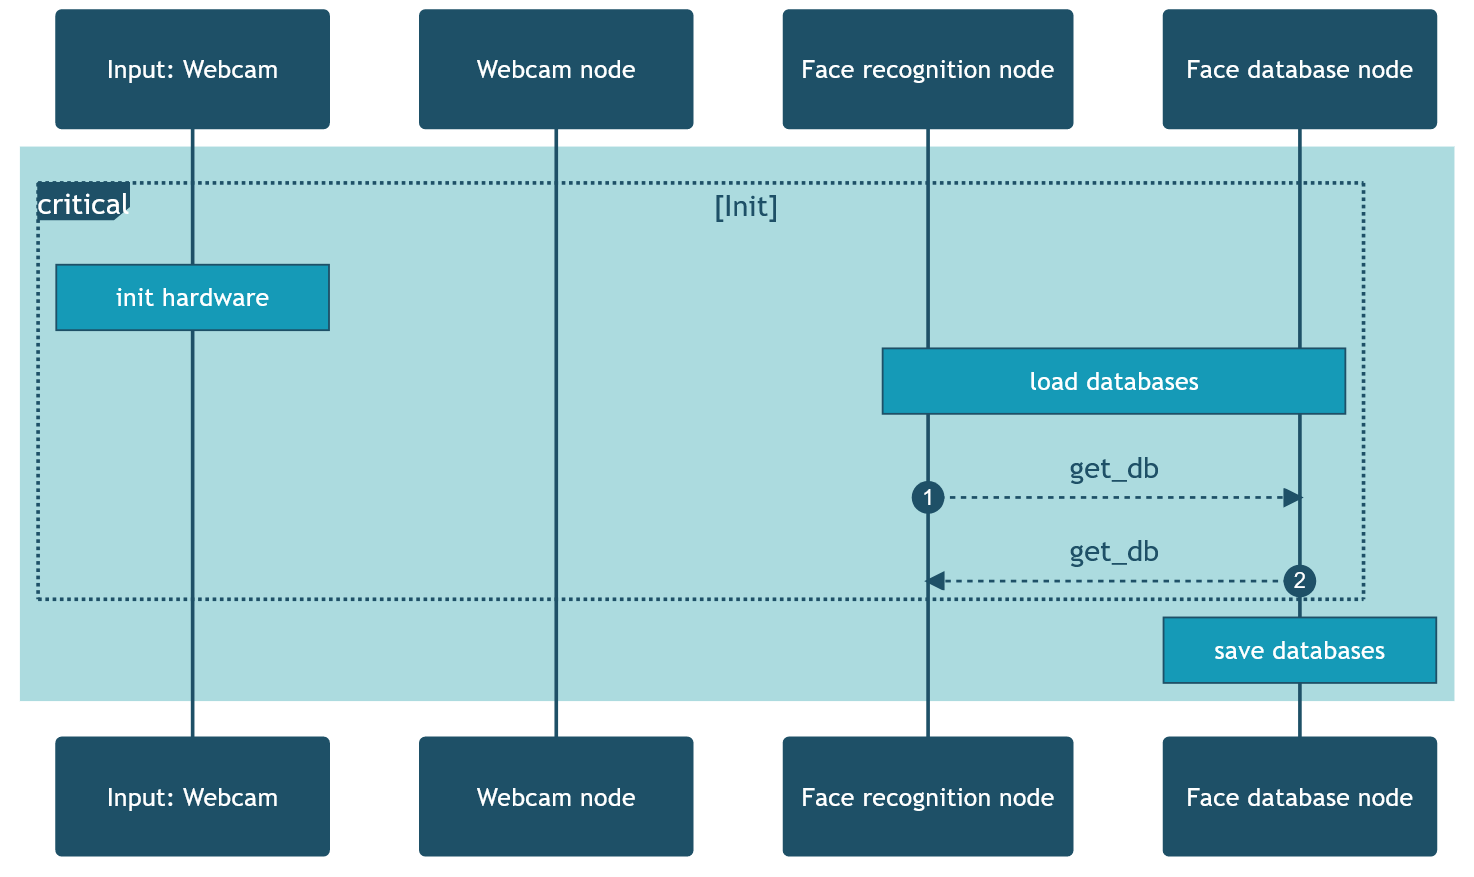
\includegraphics[width=155mm, keepaspectratio]{02_mermaid/full_init2.png}
    \caption{Csomag belső kommunikációs csatornái részletesen.}
    \label{fig:fullcomm}
\end{figure}

\clearpage
\section{Csomag moduljai}
\label{sec:modules}
    \subsection{Kamera kezelését végző node}
Az \verb|image_publisher.py| fájlban található „node” feladata, hogy a robothoz csatlakoztatott kamera élő képen Opencv-python modul segítségével végez egy elő feldolgozást, majd továbbítja a kép teljes feldolgozását, az arcok felismerését végző „node” számára.
\begin{figure}[!ht]
    \centering
    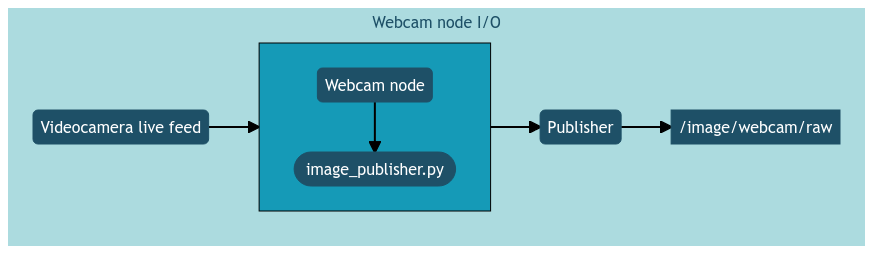
\includegraphics[width=125mm, keepaspectratio]{02_mermaid/mermaid10_wc_io.png}
    \caption{Kamera kezelő „node" „I/O"-ja.}
    \label{fig:wcio}
\end{figure}

Opencv-python modul (továbbiakban csak cv2), a nyílt forráskódú OpenCV projekt Python programozási nyelvre készült könyvtára számítógépes látáshoz, képfeldolgozáshoz. A cv2 \verb|VideoCapture| osztályának segítségével olvassa be a csatlakoztatott kamera képét, itt megadhatóak paraméterek, melyek közvetlenül befolyásolják a kiolvasott kép felbontását, enkódolását és a kiolvasás sebességét. Ezt követően a beolvasott képet át kell alakítani ROS „topic”-on publikálható formátumú üzenetté. A folyamatot a \refstruc{fig:wcp} szemlélteti. A publikálás elvégzéséhez a \verb|cv_bridge| modul segít. A modul, mint a nevéből is következik hidat biztosít a cv2-vel beolvasott kép és a ROS-ban publikált üzenet formátuma között. Az átalakítást követően az üzenetet a \verb|/image/webcam/raw| „topic”-on publikálja.
\begin{figure}[!ht]
    \centering
    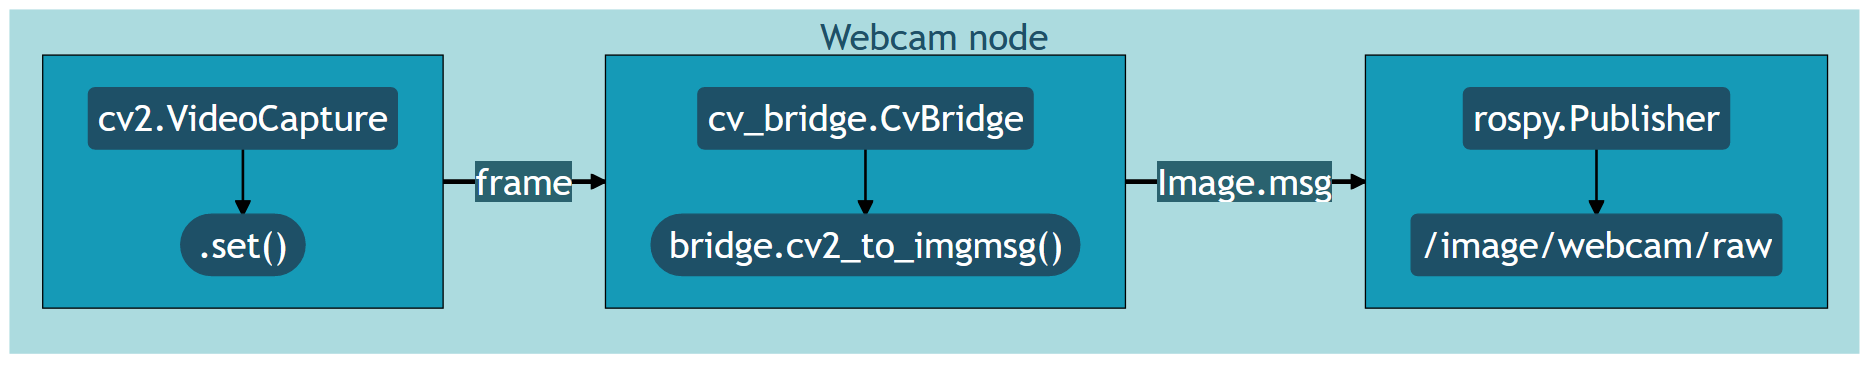
\includegraphics[width=150mm, keepaspectratio]{02_mermaid/webcam_node3.png}
    \caption{Kamera kezelő „node" folyamatábrája.}
    \label{fig:wcp}
\end{figure}

A „topic” elnevezése az általános ROS szokásjogot követi, amelyik üzenet egy képnek valamilyen enkódolását tartalmazza \verb|/image| nevű „topic”-ra kerül, ezen belül megnevezve mi a kép forrása, ami jelen esetben fejlesztés közben egy webkamera volt, illetve utólag megjelölve „raw”, aminek jelentéstartalma, hogy ez a kép teljes egészében, amit a kamera lát. Tehát még nincsenek rárajzolva az emberek arcát jelölő négyzetek és neveik.

\subsection{Arcfelismerést végző node}
Ez a „node” alkotja a csomag magját, ez a legfontosabb része, a \verb|face_recognition_core.py| fájlban implementáltam. Itt történik az emberek észlelése és azonosítása. A kommunikációhoz használt csatornáit a \refstruc{fig:frio} jeleníti meg.
%\begin{figure}[!ht]
%    \centering
%    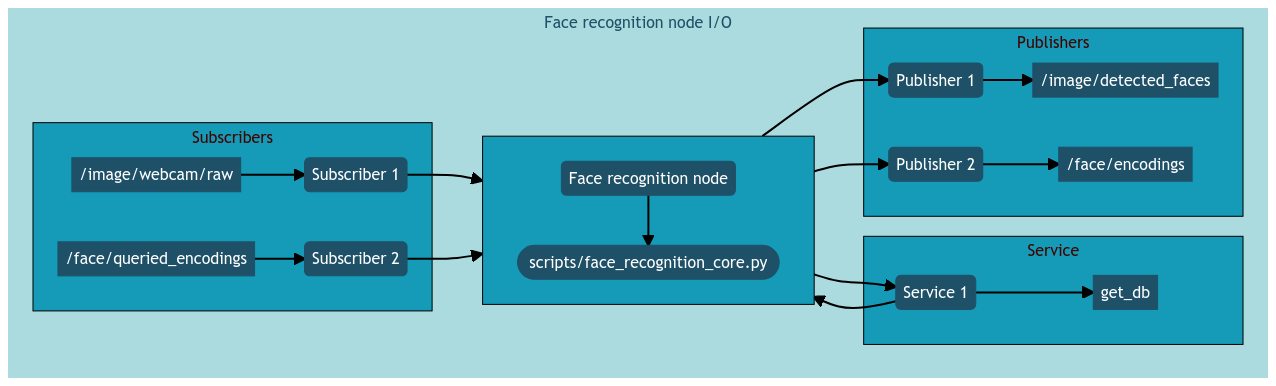
\includegraphics[width=150mm, keepaspectratio]{02_mermaid/mermaid20_fr_io.png}
%    \caption{Arcfelismerést végző „node" „I/O"-ja.}
%    \label{fig:frio}
%\end{figure}
%TODO: ábraleírás van ennyi annyi subja pubja mik a topicok

\subsubsection{Bemenetek}
Arcfelismerést végző „node” három bemenettel rendelkezi (\refstruc{fig:fri}). Az első „subscriber" feliratkozik a \verb|/image/webcam/raw| „topic"-ra, ahonnan megkapja a kamera képét \verb|image.msg| formátumban, amit a \verb|CvBridge| osztály \verb|.imgmsg_to_cv2()| függvénye alakít át felhasználható, elemezhető adattá. A második „subscriber" az adatbázist kezelő „node" által indított kommunikáció fogadására szolgál. Általam definiált \verb|Encodings.msg| formátumban megkapott adatokat a szintén általam írt \verb|DataInterface| osztály \verb|.msg2enc()| függvénye fordít a „node"-ban futó kód működéséhez szükséges formátumúvá. A „subscriber"-ek mellett kliensként is működik, a \verb|get_db| „service"-en keresztül kéri le az adatbázist kezelő „node"-tól az adatokat, itt szintén szükséges egy átalakítás, mint a második „subscriber"-ről érkező adatok fogadása során. Az alsó ábrán (\refstruc{fig:fri}) látható, hogy a \verb|DataInterface| osztály által átalakított adatok milyen formátumúak.
\begin{figure}[!ht]
%TODO szétdarabolni az ábrát NEM
    \centering
    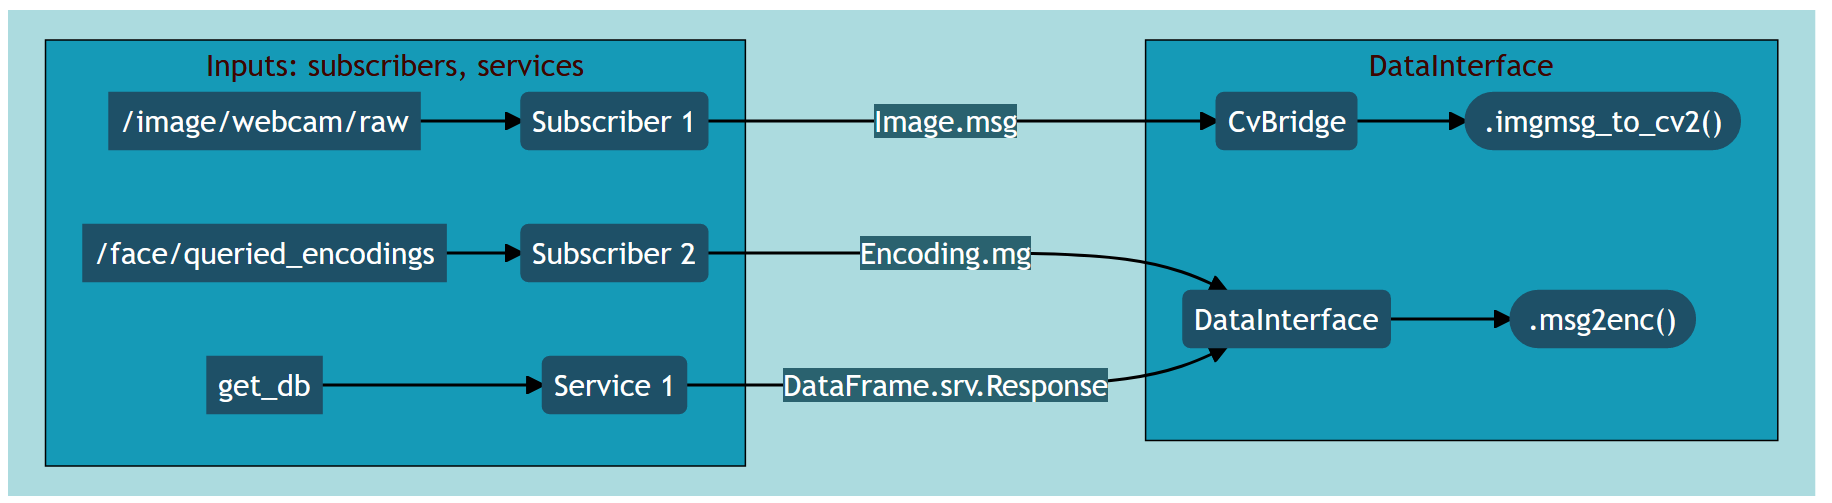
\includegraphics[width=150mm, keepaspectratio]{02_mermaid/fr_bemenet1.png}
    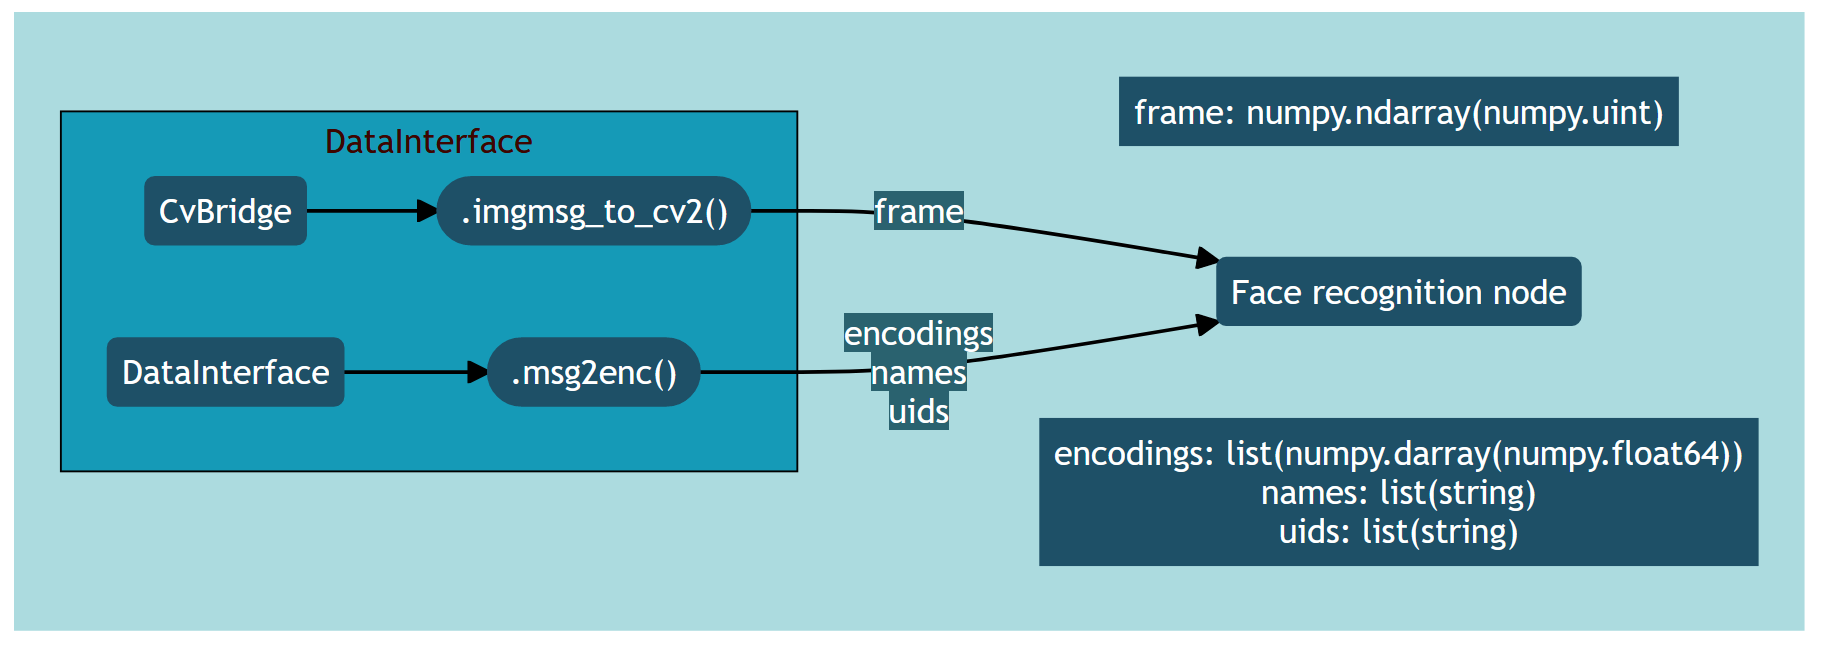
\includegraphics[width=151mm, keepaspectratio]{02_mermaid/fr_bemenet2.png}
    \caption{Arcfelismerést végző „node" bemenetei.}
    \label{fig:fri}
\end{figure}

\subsubsection{Kimenetek}
A „node" kettő „publisher"-rel rendelkezik (\refstruc{fig:fro}), amelyből az első szolgál az arcokat megjelenítő kép továbbításáért. A második „publisher" a felismert emberek arcának adatait adja át az adatbázist kezelő „node" részére. Egy „service"-t ér el kliensként, amin keresztül lekérheti a szükséges adatbázist. 
\begin{figure}[!ht]
    \centering
    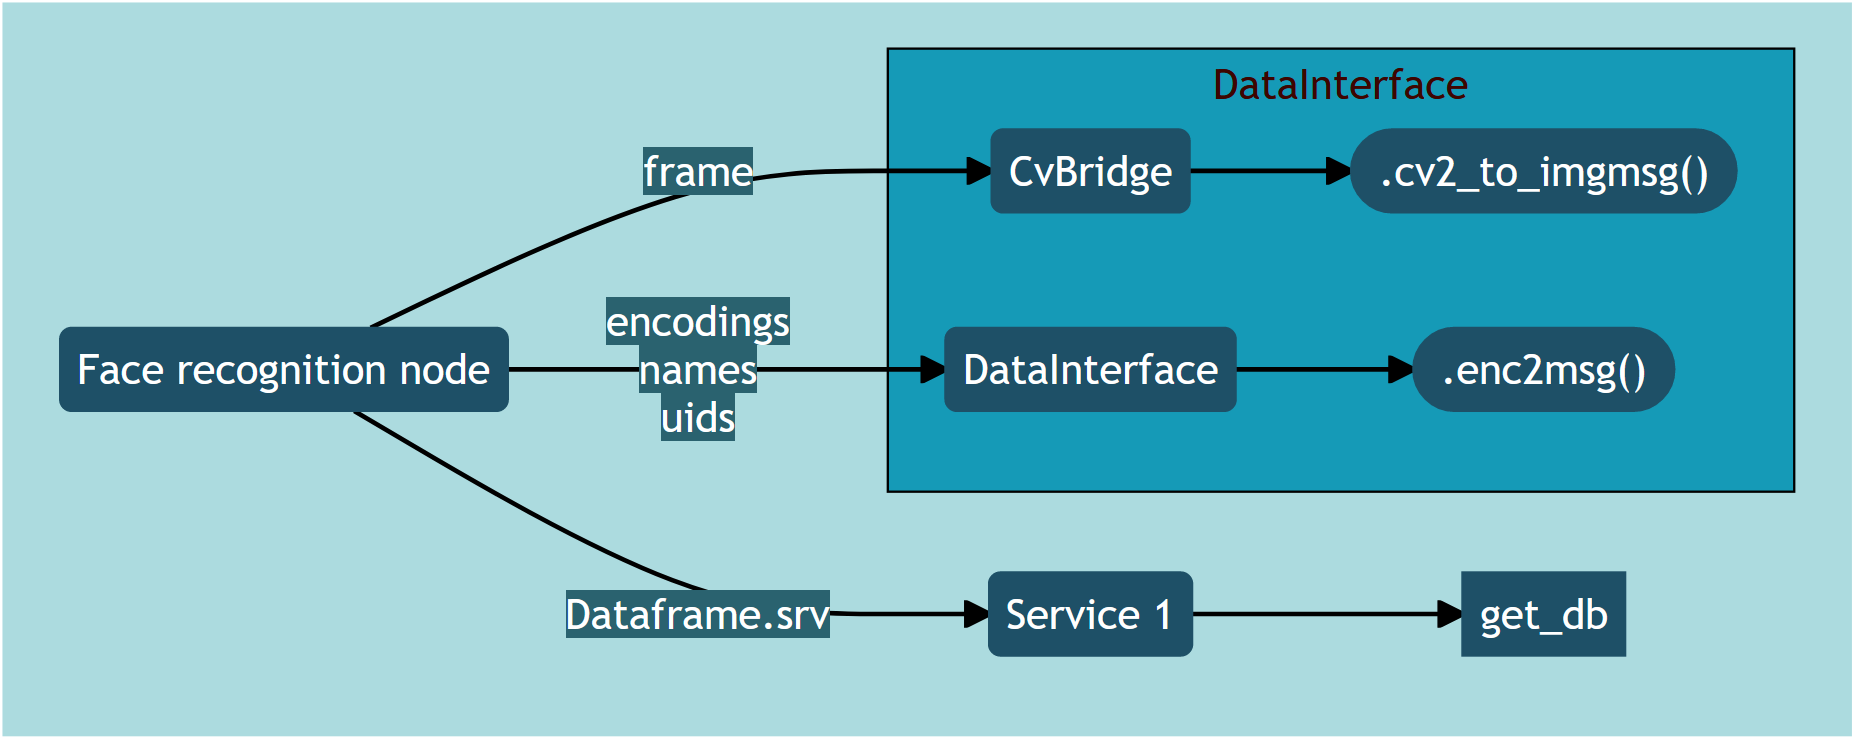
\includegraphics[width=150mm, keepaspectratio]{02_mermaid/fr_kimenet1.png}
    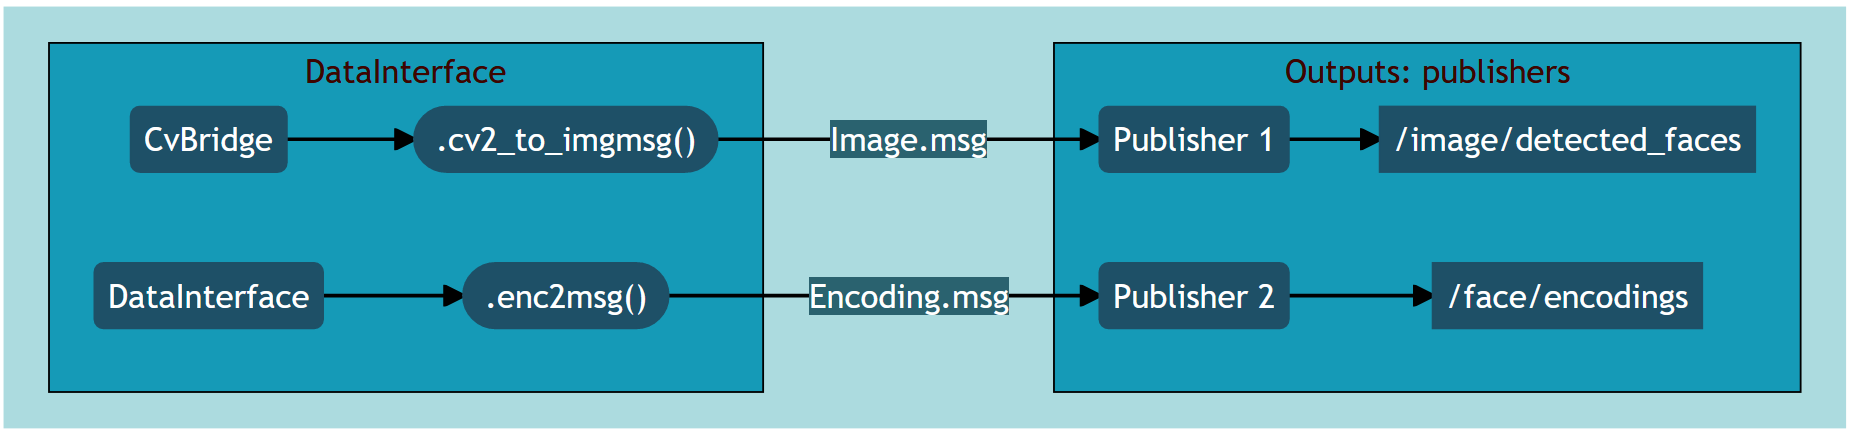
\includegraphics[width=150mm, keepaspectratio]{02_mermaid/fr_kimenet2.png}
    \caption{Arcfelismerést végző „node" kimenetei.}
    \label{fig:fro}
\end{figure}

\subsubsection{Részletes működés}
%todo mellékletben ábrát berakni initről
A „node” inicializálásakor példányosítja az \verb|ImageProcessor|-t és a \verb|DataInterface|-t. Az \verb|src/image_processor.py| fájlban van az \verb|ImageProcessor| osztály, amit a képkockák feldolgozására írtam. A \verb|DataInterface| osztályt a \verb|src/data_interface.py| fájlban implementáltam a gyakran előforduló adattípusok közötti konverzió lekezelésére. Ezeket közös „namespace”-be fordítom, így a csomag össszes „node”-jából elérhetőek. Ezekről részletesebben a következő fejezetben írok. Szintén az \verb|inti(self)| függvényben beállítom az arcok észlelésénél szükséges tolerancia értékét 0.6-nak választottam. Itt fut le egy kérés az adatbázist biztosító „node” felé, amiben lekérem az indításhoz szükséges adatbázist. Az adatbázis kialakítást részletesen az adatbázis „node” fejezetében fogom tárgyalni. Az arcfelismerést végző „node” működésének megértéséhez a lényeg, hogy létezik egy kisméretű adatbázis az adatbázist kezelő „node”-on belül, melyben megadható azon emberek arcainak enkódolása, akikkel potenciálisan gyakran találkozik a robot. Ezt az adatbázist egy „request”-en keresztül kéri le, és tölti fel a benne található adatokkal a „cache”-t. Ennek gyakorlati célja, hogy a mindenkori bemenetként szolgáló képen észlelt arcokat először ebben a „cache”-ben található arcokkal veti össze így gyorsítva a feldolgozást. A fel nem ismert arcokat a \verb|/face/encodings| „topic”-on adja át az adatbázisnak, ami elvégzi ezeknek a feldolgozását szimultán. Egyszerre fut a két „node”, így az adatbázis „node”-ban a megkapott ismeretlen arcok szortírozása nem akadályozza a kamera képének valós idejű feldolgozását.

Inicializáláskor regisztrálom a „publisher”-eket és egy „subscriber”-t, továbbá a szükséges lokális változókat.  
Az \verb|/image/webcam/raw| „topic”-ra feliratkozva éri el a webkamera képét. Minden „topic”-on megjelenő üzenet után meghívja a „callback” függvényét (\refstruc{fig:fcb}), amiben először „cv\textunderscore bridge" segítségével visszaalakítja az üzenetet egy olyan adattípusra amin már el tudja végezni a feldolgozással járó műveleteket. 

\begin{figure}[!ht]
    \centering
    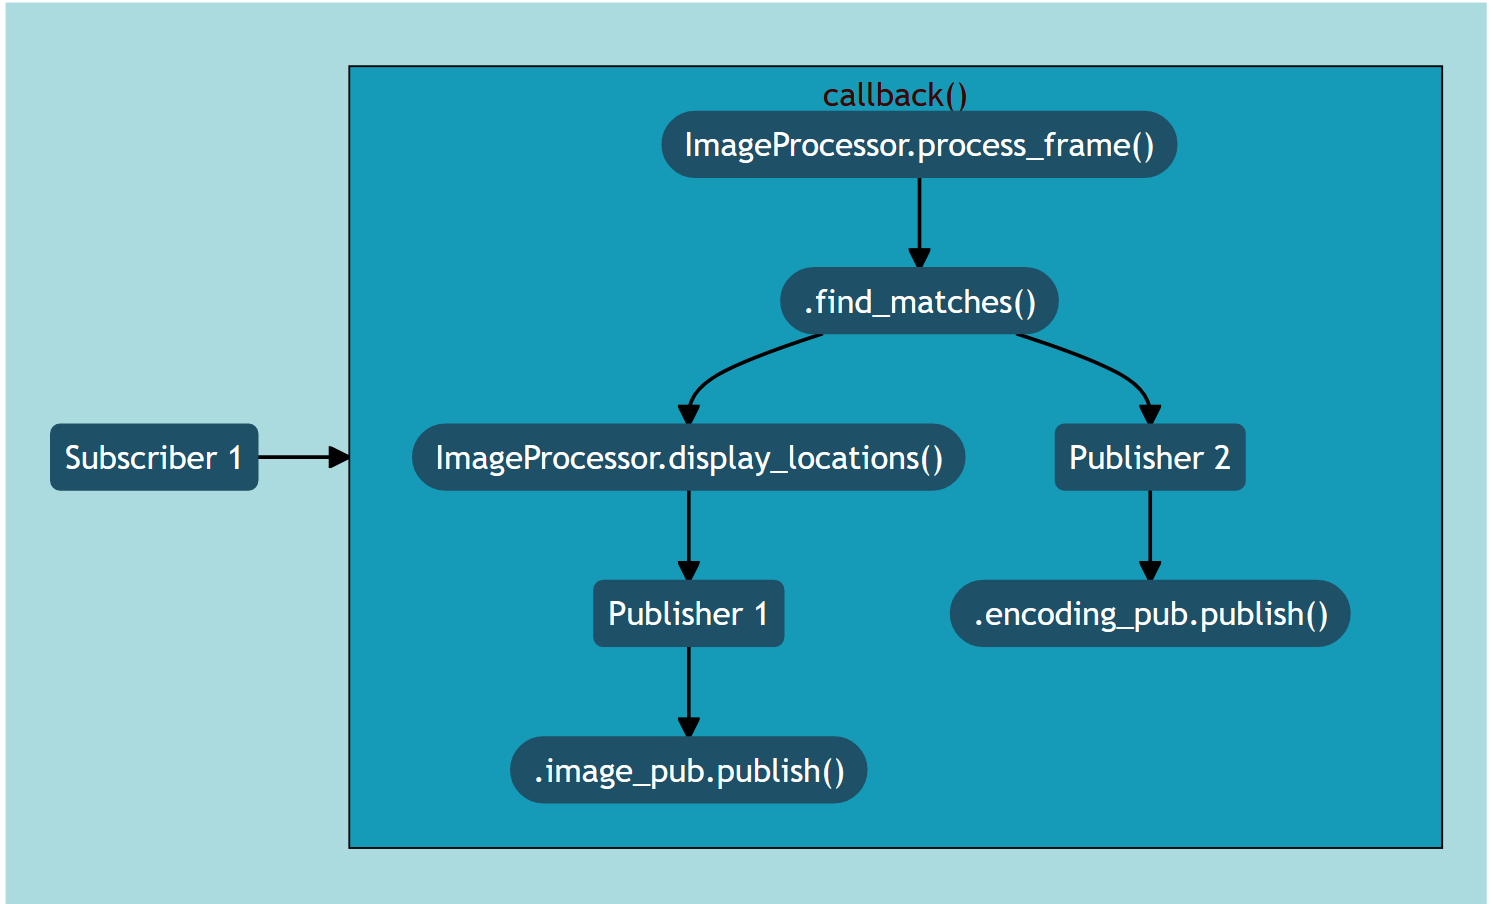
\includegraphics[width=125mm, keepaspectratio]{02_mermaid/face_callback.png}
    \caption{Arcfelismerést végző „node" „callback" függvényének működése.}
    \label{fig:fcb}
\end{figure}

Az üzenet átalakítása után a kapott képkockán először az \verb|ImageProcessor| osztály segítségével \verb|.process_frame()| függvénnyel elvégez egy arc keresést, amely visszaadja az adott képkockán található emberi arcok helyét és enkódolását. Ezt minden másik képkockán végzi el, csökkentve a hardver terhelését. A rendszer működésének tekintetében, mivel másodpercenként 25 képkockát rögzítünk (tesztelés során) ezért van bőven elég adatunk arról, hogy kiket lát a robot, szóval a teljes folyamat szempontjából jelentéktelen, hogy minden második képkockát kihagyunk. Az arcok lokációja és enkódolása egy-egy lista, amely elemszáma a képen észlelt emberi arcok száma. A helyszín lista elemei is listák. Egy arc helyét egy köré rajzolható téglalappal lehet legegyszerűbben definiálni, amit négy „integer” számmal határozza meg a „face-recognition” modul: kettő koordinátával, amik egy csúcsot jelölnek (bal felső csúcspont) és a téglalap két oldalának hosszával. Az enkódolás szintén két dimenzióban értelmezhető, az egyik dimenzió az észlelt arcok száma, a másik 128 darab „float64” típusú számból álló lista. Ezek a 128 elemű listák írják le az egyénre jellemző vonásokat. Hogy ezen belül melyik szám mit jelent, arról nincs információnk, mert ezeket egy konvolúciós háló állítja elő, aminek a belső működése számunkra egy fekete-doboz. Ugyanakkor ez a működés jelen esetben nem is jelentene semmilyen plusz információt, csupán azt az egy dolgot kell tudnunk, hogy két 128 elemű lista annál jobban fog egymáshoz közelíteni, minél jobban hasonlítanak az arcok. Ha két különböző képen ugyanazt az embert látja, akkor közel ugyanazt a 128 elemű listát kapjuk vissza. Ezen alapul az arcok összehasonlítása.

Az arcok lokációinak és „enkódolásainak” birtokában még az eredeti „callback”-en belül elvégez egy arcfelismerést. Az összes észlelt arcot összehasonlítja az összes „cache”-ből betöltött arccal. Ezt az összehasonlítást a \verb|find_matches()| függvény végzi. Végig iterál a „cache”-ben tárolt arcokon és mindegyikkel összeveti az észlelt arcokat a \verb|face_recognition.compare_faces()| függvénnyel. A ciklus annyiszor fut le ahány arcot talált a program a képen. Minden ciklusban a fenti függvény kimenete egy „boolean” lista. A tárolt arcok sorrendjének megfelelően igazat vagy hamist ad annak függvényében, hogy a beállított tolerancia érték szerint hasonló arcot talált-e. Szintén ugyanebben a ciklusban, amiben az észlelt arcok listájából egyet vet össze az összes eddig eltárolt arc információjával, megvizsgálja milyen távolságra van tőlük \verb|face_recognition.face_distance()| függvényben. A távolságot euklideszi térben kell értelmezni. Már említett módon, a konvolúciós háló ad bármely arcról egy 128 elemű listát. Gyakorlatilag egy 128 dimenziós térben számolja a függvény a távolságot. Az arcok összehasonlításának egy lista lesz az eredménye, mely tartalmazza rendre a tárolt arcoktól való távolságát, ami azt reprezentálja mennyire hasonlít hozzájuk. Ezt a listát összevetve azzal, amiben azt tároljuk, hogy melyik arc reprezentál találatot, a találatok közül ki tudjuk választani azt, aminek a legkisebb a távolsága a vizsgált arctól.

A \verb|find_matches()| függvény az észlelt arcokat kettőféleképpen csoportosítja: felismert, ezeket ellátja az adatbázisból kiolvasott névvel, illetve nem felismert „Unknown”, az olyan arcok akikkel nem talált egyezést a betöltött „cache”-ben. A függvény kimenete két lista: nevek és „uid"-k, mindkettő az észlelt arcok „enkódolásait” tartalmazó lista sorrendjének felel meg. A név lista értelemszerűen az „enkódoláshoz" tartozó név változókat tárolja „string” formátumban. A „uid” listában, szintén „string” adattípusban annak az arcnak az egyedi azonosítóját tartalmazza, amihez a vizsgált „enkódolás" legközelebbi egyezést talált. Ez pedig arra szolgál, hogy miután a „node” átadja az adatbázis-t kezelő „node”-nak a listákat a feldolgozás során tudja növelni egyel az értékét a megfelelő archoz tartozó találat számláló mezőnek.

A \verb|find_matches()| függvény visszatérési értéke egy „boolean” változó, a függvény elején vizsgálom, hogy a helyszíneket tartalmazó lista hosszabb-e, mint nulla azaz, talált-e arcot. Ha nem akkor nem is végzi el az összehasonlításokat és hamis értékkel tér vissza. Ha hosszabb a lista, mint nulla, tehát az előző \verb|ImageProcessor.process_image()| függvény észlelt emberi arcot, akkor elvégzi az összehasonlítást és felülírja az osztályváltozóként deklarált nevekből és „uid”-kból álló listákat. Ezt a visszatérési értéket vizsgálom a következő lépésben. Az arcokat a képkocára rajzoló függvény az \verb|ImageProcessor.display_faces()| csak akkor fut le, ha észlelt arcokat a program. Ennek a kivitelezésnek az oka a spórolás az erőforrásokkal. Egyértelmű, hogy ha nem észleltünk arcokat nincs szükség azok kirajzolására, tehát felesleges meghívni a \verb|.display_faces()| függvényt. Abban az esetben, ha észleltünk arcokat és meghatároztuk a nevüket, legyen ismert név vagy nem ismert „Unknown”, kirajzoljuk a „locations” listában található koordináták alapján az arcokat jelölő téglalapot és aláírjuk a hozzátartozó nevet. Háromféle kategóriát különítek el a kirajzolásnál. Az első a névvel felismert arcokat  zöld színnel, a felismert, de név nélküli „Unknown\textunderscore id” arcokat kékkel és a még nem osztályozott „Unknown” arcokat pirossal rajzolja ki a függvény. A képkockára rárajzolás után a módosított képkockát publikálom az \verb|/image/detected_faces| „topic”-on. A „topic”-ra való közlést megelőzi egy átalakítás a \verb|CvBridge.cv2_to_imgmsg()| segítségével. Gyakorlatilag a kép üzenet formátumot fogadó „callback” függvény egy üzenet adattípusban kapja meg a képet, amit vissza alakít cv2-ben és „face-recognition"-ben feldolgozható képpé, majd a feldolgozást követően visszaalakítja üzenet formátumba, hogy ROS keretrendszerben elküldhető legyen.

Ezt a publikálást minden „callback” híváskor végrehajtom, hogy a kimeneti kép folyamatos legyen. Ugyanakkor beépítettem, már fentebb kifejtett módokon, az erőforrásokkal való spórolás céljából különböző ellenőrző lépéseket, tehát nem minden „callback” híváskor módosul az üzenetként megkapott kép. Ha nem talál arcot, akkor ugyanazt a megkapott képet továbbítja, csak egy különböző „topic”-ra. A kép publikálása után, ami minden hívásban megtörténik, implementáltam még egy publikálást, amiben nem képet, hanem az azon észlelt majd felismert arcokhoz tartozó információkat („enkódolás", név, „uid”) listákat küldöm a \verb|/face/queried_encodings| „topic”-ra. Ez az adatbázis kezelő „node” számára való információ átadás csatornája. Itt két erőforrás felhasználást csökkentő lépést iktattam be. Egyrészt vizsgálom, hogy talált-e emberi arcot a képen, ha nem akkor felesleges elküldeni a nulla elemeket tartalamazó listákat. Másrészről egy időzítő osztályváltozót hoztam létre, ami 25 „callback” hívásonként engedélyezi csak a közlést a „topic”-on. Erre azért van szükség, mert az adatbázist kezelő „node” erre a „topic”-ra feliratkozott „callback” függvényének a futásideje hosszú és műveletigényes. Ha emberi viselkedéshez akarjuk hasonlítani, itt történik meg az, amikor meglátunk egy arcot, nem jut eszünkbe a személy neve, és elkezdünk rajta gondolkozni. Nincs szükségünk arra, hogy másodpercenként 25 képet alkossunk arról az arcról, elég egyszer „ránéznünk" (mintavételeznünk). Így implementáltam a programban is. Ha 25 képenként, azaz 1 másodpercenként (mivel 25 fps-el rögzít) látunk egy emberi arcot, akkor már elkészíti róla az „enkódolást", amit átadhat az adatbázisnak a bővebb felismerés lefolytatásához. De erről a folyamatról részletesebben az adatbázis kezelő „node” leírásában írok.

\subsection{Arcok észlelését végző osztály}

Ebbe az általam írt osztályba szerveztem ki az arcok felismerését és képkockára rajzolását. A csomag kimenete az élő webkamera kép, rajta az arcok helyét jelölő kerettel és a keret alatt egy négyzetben az emberek nevével.
Osztályváltozóként lehet megadni a színkódokat; három különböző színnel ad visszajelzést, ami az emberek felismertségét jelenti. Zöld színnel az inicializáláskor megtanított emberek arcát jelöli, akikhez név is társul, kékkel az egyszer már látott és elmentett arcokat, ahol a név: „Unknown\textunderscore id” és a még nem elmentett, először látott arcokat pirossal és „Unknown” névvel.

Az osztály két fügvénnyel rendelkezik, az első: a \verb|.process_frame(frame)|, ahol a \verb|frame| változóban megadott képkockán végzi el az arcok keresését. Először a megadott \verb|factor| értékkel méretezi át a képet. Ez a lépés erőforrás optimalizálás céljából indokolt. Kisebb kép is tartalmazza ugyanazt az információt az arcokról, ami szükséges a sikeres felismeréshez, de kisebb méretű képet hamarabb dolgoz fel az algoritmus, kevesebb erőforrás igény mellett.  Ez után a képet át kell alakítani RGB formátumra. A cv2 modul által rögzített képkocka egy több dimenziós mátrix, ahol minden pixelnek van három szín értéke, melyeket nem piros-zöld-kék sorrendben tárol, hanem kék-zöld-piros sorrendben, mely a modul sajátossága. Viszont a „face-recognition” modul számára RGB formátumú képre van szükség. Az áttranszformálás után ez az első függvény megkeresi az arcok helyét, amit egy egy dimenziós listaként kapunk meg, majd a helyek segítségével megalkotja az arcokhoz tartozó enkódolást. Ez egy „n” dimenziós lista, ahol „n” az arcok száma és mindegyik eleme egy 128 elem hosszúságú lista, ami az arcok reprezentációjára szolgáló vektor értékeit tárolja. A függvény kimenete a helyszín lista és az enkódolások listája.

A második függvénye az osztálynak a \verb|.display_locations()|. A függvény argumentumai: \verb|frame| – a képkocka amire rajzol, \verb|locations| – az arcok helyei a képen, és a \verb|names| – az arcok nevei. Mivel az arcok koordinátáit méretezett képen határoztuk meg, ezért át kell őket transzformálni, ez egy szorzást jelent a \verb|.process_frame()|-ben használt tényező reciprokával. A kapott koordinátákkal a cv2 modul \verb|.rectangle()| és \verb|.text()| függvényeivel a képkockára rajzolja az arcok köré a keretet a megfelelő színnel és alá írja a neveket. A függvény a módosított képkockával tér vissza. Paraméterek, amiket tetszés szerint meg lehet választani: betűtípus, betűméret, színek, keret vastagsága.

\subsection{Adatbázis}
Az adatbázis 6 oszlopból épül fel (\refstruc{tab:adatb}) és minden arcról készített enkódolás külön sort képez. „Name” oszlopban a személy neve, arcának „enkódolása” pedig a „Face” oszlopban van. Minden archoz tartozik egy egyedi „uid” (az „Id" oszlopban), ennek az azonosítás és az adatok megkülönböztetésének szempontjából van szerepe. A „Folder” és „Filename” oszlopok azon „enkódolásokhoz" tartozó fájlok és mappájuk nevét jegyzik, amik a csomag \verb|images| mappájában találhatók. Az új látott arcok feldolgozása során az adatbázis korábbi adataival hasonlítja össze őket, és számolja, hogy melyiket találta optimális egyezésnek. Ezt az adatot a „Matchcounter” oszlop gyűjti, egy egész „integer” számmal jelöli hányszor bizonyult találatnak egy adott enkódolás az összehasonlítás folyamán. Ahányszor pozitív egyezést talál megnöveli egy számmal. Innen lehet következtetni arra, hogy mely enkódolás a legpontosabb egy arcról.
\begin{table}[!ht]
	\footnotesize
	\centering
	\begin{tabular}{ l c c }
		\toprule
		Elnevezés & Jelentés & Típus \\
		\midrule
        Name & archoz tartozó név & string\\
        Id & uid & string\\
        Folder & mappa neve & string\\
        Filename & fájl neve & string\\
        MatchCounter & egyezések száma & integer\\
        Face & enkódolás & list\\
		\bottomrule
	\end{tabular}
	\caption{Az adatbázis oszlopai.}
	\label{tab:adatb}
\end{table}

Mivel az adatbázis minden elemét meg kell különböztetnünk egymástól, ezért kell egy attribútum, ami alapján ezt elvégezhetjük. A név nem egy jó választás, mivel egy ember arcáról több „enkódolást" is le tudunk menteni. Mappa és fájlnév sem használható, mert ezzel csak az adatbázis inicializálásakor betöltött enkódolások rendelkeznek. Ezért hoztam létre egy külön „Id” oszlopot amiben a Python egy moduljának \verb|uuid.uuid4()|\footnote{python uuid: \url{https://docs.python.org/3/library/uuid.html}} függvényével generálok egy véletlenszerű azonosítót RCF4122 szabvány\footnote{RCF4122 szabvány: \url{https://www.rfc-editor.org/rfc/rfc4122}} szerint. Ezt utána „string”-ként tárolom, mivel ilyen formában át tudom adni „message”-eken és „service”-eken keresztül. Mivel ROS-on belül nincs „uuid” osztály, ezért csak „string”-re átalakítva tudom „node”-ok között átvinni. Logikátlan lett volna, ha nem „string”-ként tárolom, mivel rendszeresen oda és vissza kellett volna alakítanom. Így egyszer létrehozáskor átkonvertálom „string”-é és utána bármikor használható és összehasonlítható lesz.



%TODO: „uid” – stringben tárolás könnyű összehasonlítás python példa jupyter notebook
%TODO2: táblázat az adatoknak
%Name (név): string
%Id (egyedi azonosító): string
%Folder (mappa): string
%Filename (fájlnév): string
%MatchCounter (találatok száma): int
%Face (arc kódja): tömb valami…

\subsection{Adatbázist kezelő node}
A \verb|face_database.py| fájlban található \verb|FaceDatabase| „node" feladata, hogy adatbázist biztosítson az arcokról készített enkódolások tárolására. Adatbázis gyanánt a Pandas modul \verb|DataFrame| osztályát használom, amit a könnyű kezelhetősége és kis tárhely igénye miatt választottam. További előnyei, hogy nincs szükség külön adatbázis például MySQL futtatására. Mindezek mellett fontos tervezési lépésként úgy döntöttem, hogy készítek egy \verb|DatabaseManager| osztályt, ami abban a tekintetben bonyolít a csomag felépítésén, hogy egy plusz architekturális réteg került bevezetésre. Előnye, hogy ebben az osztályban a Pandas féle \verb|DataFrame| specifikus lekérdezések és adatmódosítások kicserélhetőek másik adatbázis kezelő moduléra. S mivel az adatbázist kezelő „node”-ban nincsenek közvetve meghívva a \verb|DataFrame| osztály tagfüggvényei, a saját \verb|DatabaseManager| osztály függvényeit használja. Ennek a tervezési döntésnek köszönhetően nem jelentene semmilyen problémát, ha másik adatbázis kezelőre cseréljük ki. 

A „node” a ROS-on belüli kommunikációhoz egy „subscriber”-t, egy „publisher”-t használ (\refstruc{fig:dbio}). A \verb|/face/encodings| „topic”-ra feliratkozott „subscriber”-rel kapja meg az élő kamera képén észlelt, felismert emberek arcainak enkódolását, neveit, „uid”-ját. A \verb|/face/queried_encodings| „topic”-on publikálja a lekért emberekhez tartozó arcok neveit. Egy „service” biztosítja az indításkor a „face-recognition” „node” felé a kezdő adatbázis lekérését.

\begin{figure}[!ht]
    \centering
    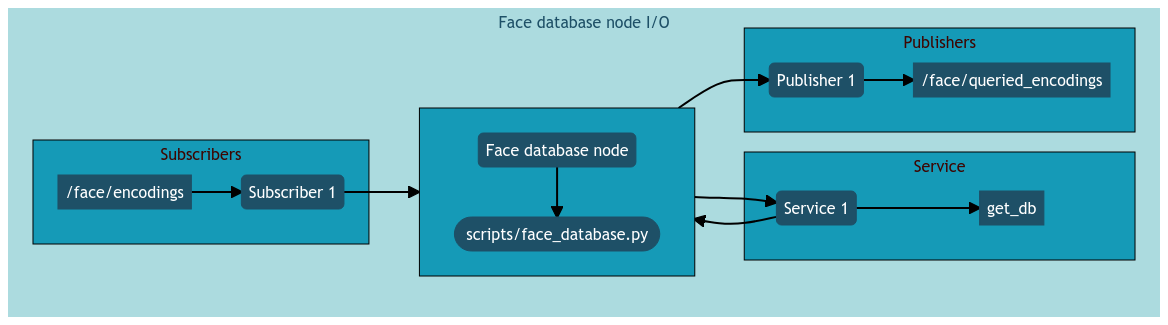
\includegraphics[width=150mm, keepaspectratio]{02_mermaid/mermaid30_db_io.png}
    \caption{Adatbázist kezelő „node" „I/O"-ja.}
    \label{fig:dbio}
\end{figure}

\subsubsection{Bemenetek}
Az adatbázis kezelő „node” a bevett szerver-kliens architekturális elrendezésben szerverként viselkedik, mellyel lekérhető futásidőben az adatbázis. Jelenleg a működés szempontjából lényeges kezdő adatbázis lekérésre van lehetőség. A \verb|get_db| név alatt kínál egy meghívható „service”-t amit bármelyik „node”-ból le lehet kérni, ez a funkcionalitás is a ROS alapelveinek köszönhető. A csomag robotra illesztésekor ennek köszönhetően más csomagok „node”-jaiból indított „request”-el el lehet kérni az adatbázist, ha erre szükség lenne. A csomagomban jelenleg egy „node”-ban implementáltam a hívást. A „face-recognition” „node” küldhet „request”-et az adatbázis kezelő „node”-nak amellyel inicializáláskor áttölti a kezdő adatbázis tartalmát a saját „cache”-be.

A \verb|/face/encodings| „topic”-ra feliratkozott „subscriber” felelős azért, hogy az arcokat felismerő „node”-ban erre a „topic”-ra küldött adatokat beolvassa. Minden publikált adatcsomagnál meghívja a „callback” függvényt, ami feldolgozza ezeket. Mivel ROS-on belül nincs lehetőség több dimenziós lista vagy tömb elküldésére, ezért egy dimenziós formában érkeznek az adatok, amiket a \verb|DataInterface| osztály \verb|.msg2enc()| függvényével alakítja vissza a megfelelő formátumra.

\begin{figure}[!ht]
    \centering
    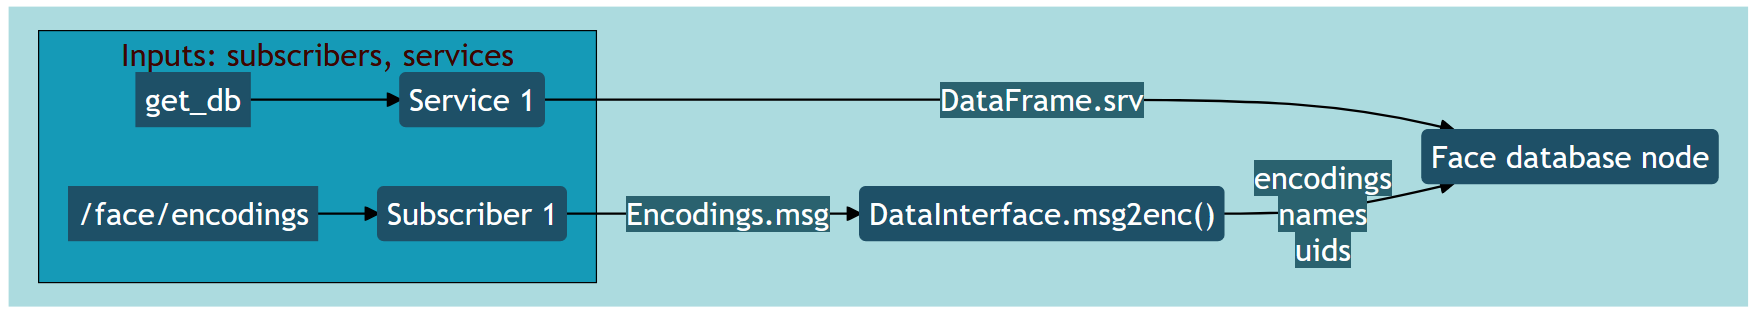
\includegraphics[width=150mm, keepaspectratio]{02_mermaid/db_bemenet1.png}
    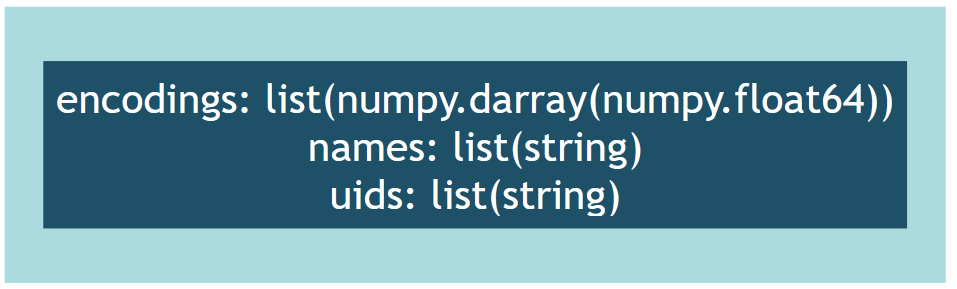
\includegraphics[width=70mm, keepaspectratio]{02_mermaid/db_bemenet2.png}
    \caption{Adatbázist kezelő „node" bemenetei.}
    \label{fig:bdi}
\end{figure}

\subsubsection{Kimenetek}
A \verb|get_db| „service” az előző fejezetben leírtak szerinti meghívásakor küldi el a szükséges adatokat. Emellett a „publisher” biztosítja a lekért arcokhoz tartozó adatok publikálását az arcfelismerést végző „node” felé. Itt szintén a \verb|DataInterface| osztály felhasználásával fordul le az adatbázis struktúrájának megfelelő tartalom.
\begin{figure}[!ht]
    \centering
    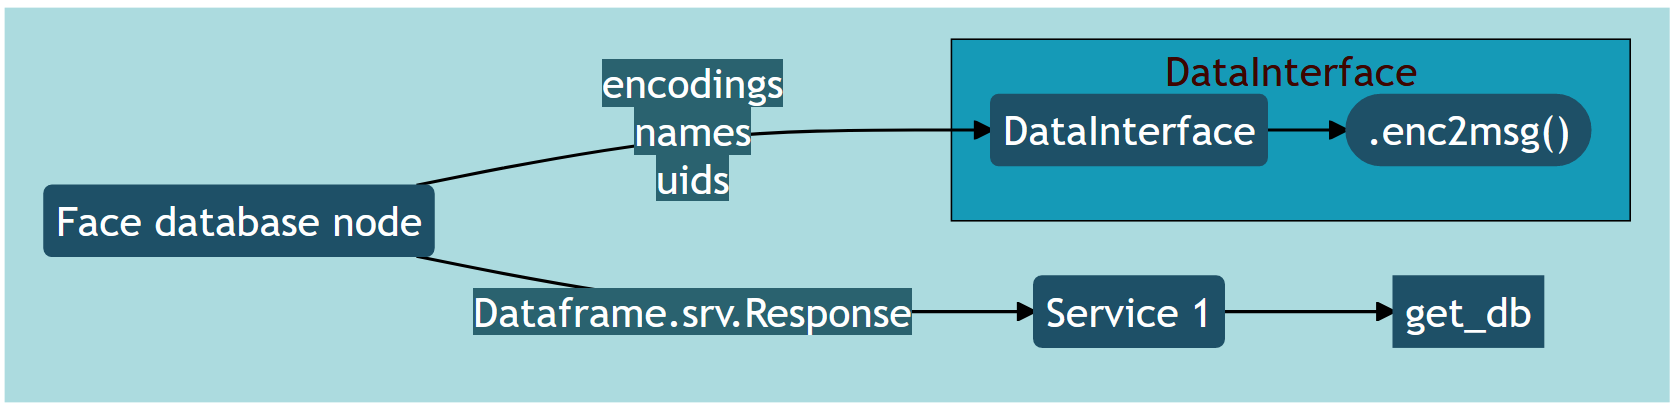
\includegraphics[width=150mm, keepaspectratio]{02_mermaid/db_kimenet1.png}
    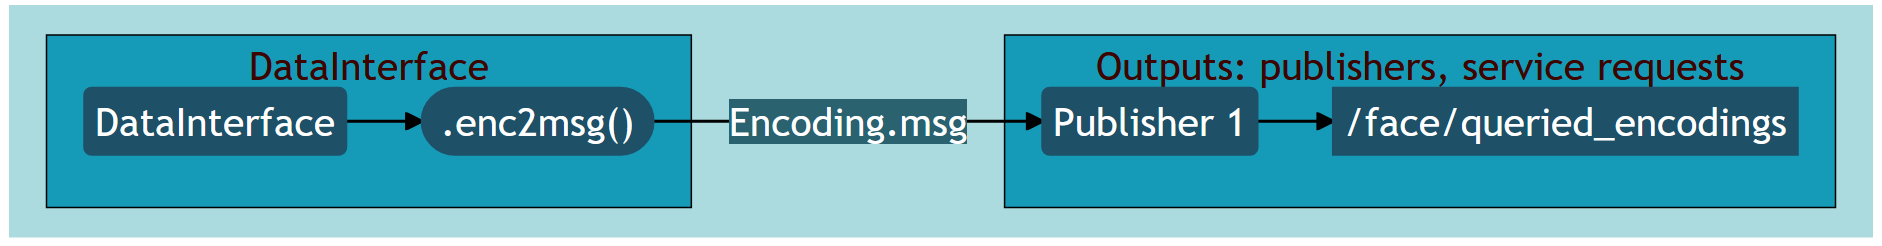
\includegraphics[width=150mm, keepaspectratio]{02_mermaid/db_kimenet2.png}
    \caption{Adatbázist kezelő „node" kimenetei.}
    \label{fig:dbo}
\end{figure}

\subsubsection{Részletes működés}
A \verb|face_database.py| \verb|main| függvénye a szokványos felépítést követve először inicializálja a „node”-ot, majd a megadott „rate” frekvencia értékkel futtatja \verb|rospy.spin()| fügvénnyel. A „FaceDatabase” osztály a „node” implementációjának kezdésekor beállítja az osztály változóit, inicializálja a „subscriber”-t és „publisher”-t. Valamint létrehozza az adatbázisokat. Leállításakor elmenti a használt adatbázist.

A függvény három adatbázist hoz létre. Az első „Start” vagy kezdő adatbázis, ezzel töltődik fel a „face-recognition”-ben a „cache”. Ez az az adatbázis, amely azon a kulcsfontosságú emberek adatait tartalmazza, akiket előreláthatólag gyakran kell felismernie a robotnak. Az arcfelismerést végző „node” először ebben az adatbázisban kutat egyezés után, ha nem talál, akkor adja át az adatbázist kezelő „node”-nak az észlelt arcok „enkódolását”. A második és harmadik adatbázis megegyezik tartalom tekintetében inicializáláskor. Mint az a kódban is látható, a „Main” vagy fő adatbázist fájlból olvassa ki és utána a futásidőben használt „live\textunderscore df” vagy élő adatbázis adatait innen másolja ki. A programkód futás közben ezt a „live\textunderscore df” adatbázist módosíthatja csak, a fő adatbázist nem tudja szerkeszteni. Azért ezt a megoldást használom, mert előnyös, hogy ha van egy olyan adathalmaz, amihez bármilyen meghibásodás, vagy zavar esetén vissza tudunk térni. Ennek a funkciónak az implementálására azért volt szükség, mert a \verb|pandas.DataFrame| osztály nem rendelkezik beépített biztonsági mentés kezelő funkcióval. Az adatbázisok kezelésére írt \verb|DatabaseManager| osztály inicializálja az adatbázisokat. Ha nem találja a fájlokat, akkor létrehozza és feltölti őket a rendelkezésre álló adatokkal. Ezeket az adatokat képekből nyeri ki, amelyeket megadhatunk a csomag \verb|/images/known_faces/| mappájában. A struktúra, amit felépítettem az arcok tárolására az alábbi: minden ismertnek titulált arcról készült képet az előző mappában személyenként külön-külön mappába kell rendezni. Lehetőség szerint a képen egy ember legyen látható, mert az algoritmus jelen implementációja szerint egy fájlt csak egy archoz tud társítani, ha több ember szerepel a képen akkor az először észlelt arcot kapcsolja a névhez. A személy nevét a mappa neve adja. Tehát, például ha \verb|/images/known_faces/mate| mappában talál a szoftver három \verb|.png| kiterjesztésű fájlt, akkor beolvassa mindegyiket, és hozzájuk a mappa nevét, azaz „mate” nevet rendeli. Az emberek elnevezése innen származik, ezt későbbieknek (a képek beolvasása után) nem lehet megváltoztatni viszont az utólagos név választás vagy módosítás funkcióját könnyen lehet implementál, egy „service” segítségével. Ez az adatbázisban egy megadott „uid”-hoz tartozó sor nevet tartalmazó mezőjét átírja a „request”-ben „string” típusban megadott értékre.

A \verb|/face/encodings| „topic”-ra feliratkozott „subscriber” meghívja az osztály „callback” függvényét (\refstruc{fig:dbcb}). Ebben a fügvényben történik az adatok feldolgozása. A megkapott adatokat a \verb|DataInterface| osztály segítségével átalakítja a  „node”, mellyel megkapja az élő kamera képről felismert emberi arcokat. Az arcokat kétféleképpen osztályozza a „face\textunderscore recognition\textunderscore core.py”-ban futó „node”.
\begin{figure}[!ht]
    \centering
    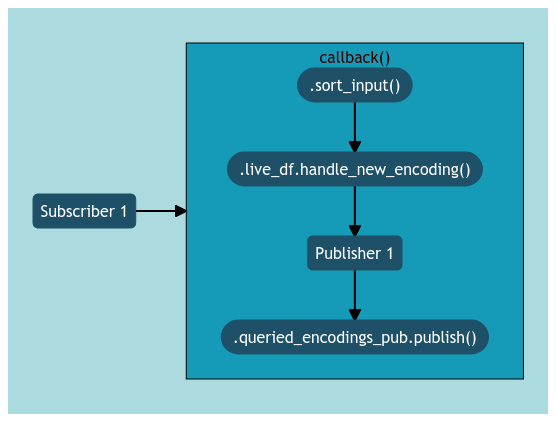
\includegraphics[width=100mm, keepaspectratio]{02_mermaid/mermaid34_db_callback.png}
    \caption{Adatbázist kezelő „node" callback függvénye}
    \label{fig:dbcb}
\end{figure}

Ha talál a „cache”-ben egyezést a felismert arcokhoz, amiket az enkódolás képvisel, akkor hozzá társítja a létező találatot jelentő ember nevét és a találat „uid”-ját. Ennek a „uid”-nak abban van szerepe, hogy a „callback” függvény így megtalálja az adatbázisból az egyezést biztosító elemet és megnövelje a „MatchCounter” mező számát. Innen lehet következtetni, hogy egy elem hányszor biztosított megfelelő felismerést. Minél közelebbi a két enkódolás, annál pontosabb az egyezés. Tehát megállapítható a „MatchCounter” száma alapján: minél nagyobb annál jobb alapot biztosított bizonyos ember felismeréséhez. Ezt követően a művelet generál egy új egyedi „uid”-t amit hozzá társít ehhez a beérkező „enkódolás”, név pároshoz és elmenti az adatbázisba. 


Ha nem talált a „cache”-ben egyezést, akkor „Unknown”-ként jelöli meg. Ez két opciót jelenthet. Az első, hogy van információnk az illetőről, de még azt nem töltöttük át a „cache”-be. A második opció, hogy valóban ismeretlen ember állt a kamera előtt. Emiatt szükséges egy összevetést végeznünk a teljes adatbázison, hogy kiderüljön létezik-e a látott ember arcához tartozó enkódolás.
Ez volt a fő tervezési gondolat a „cache” létrehozása körül. Tulajdonképpen megrövidítem azoknak az elemeknek a számát, amin végig kell iterálnia, így biztosítva az arcfelismerésre szolgáló „node” kimenetének késésének minimalizálását. Ha csak egy kisebb méretű „cache”-t kell ellenőriznie gyorsabban végez vele, mint ha az egész adatbázison tenné ugyanezt. A fel nem ismert enkódolások átadásával átszerveztem a sok feldolgozást követelő, időigényes műveletet az adatbázis kezelő „node”-ba. Itt párhuzamosan futhat és ha végzett visszatérhet aszinkron a \verb|/face/queried_encodings| „topic”-on a keresett elemekkel. Így nem lassítja az arcfelismerő „node” működését, ami ennek köszönhetően folyamatosan tud adatot biztosítani az egész csomag kimenetének tekintendő \verb|/image/detected_faces| képfolyamon.

Az „Unknown” vagy névvel ellátott enkódolások beérkezése után lefolytatott feldolgozás során megállapítom, hogy valóban ismeretlen-e a személy, vagy már a robot egy előző alkalommal találkozott az emberrel. Ha találkozott, akkor az adatbázisból kiolvassa a kód az adatait és továbbítja a „cache”-be. Ha nem ismert, azaz valóban „Unknown”, akkor generál hozzá egy id-t, ami után elmentésre kerül „Unknown\textunderscore id” névvel, egy egyedi „uid”-val és a beérkezett enkódolással. Majd az elnevezést áttölti a „cache”-be. Mivel ez aszinkron módon párhuzamosan fut le az élő kamera képen végzett észleléssel, ezért nem kizárt, hogy a következő felismerési ciklus megkezdése előtt még nem éri el az arcfelismerést végző „node” „subscriber”-re, így újra lejátszódhat az egész folyamat. Itt lehetne a csomagot még optimalizálni, oly módon, hogy az adatbázist kezelő „node” lokálisan eltárolja a lekérdezett enkódolásokat és csak akkor végzi el az újak feldolgozását, ha ebben a lokális listában nincs jelen. Ennek a kivitelezésére nem találtam optimális megoldást, mivel az ugyanarról az arcról beérkező enkódolások is különböznek: mivel két kép nem egyezik meg tökéletesen, így nincs módom egy egyszerű összehasonlítást elvégezni, amivel meghatározhatom, hogy ezt az arcot vizsgáltam-e már. Pontosabban ugyanazt az összehasonlítást tudnám elvégezni a „face-recognition” modul függvényeivel, ami amúgy is lefut a beérkező „Unknown” arcok válogatásánál. Ezért nem láttam indokoltnak, hogy egy további lépéssel bonyolítsam és lassítsam a feldolgozást. Tervezői lépés, amit ezek ellenére megtettem, hogy minimalizáljam a duplán feldolgozást, hogy a \verb|/face/encodings| „topic” publikálást kisebb frekvencián végzem, nem minden képkocka vizsgálatánál, csak minden huszonötödiknél (25 képkocka per másodperc rögzítése esetén másodpercenként egyszer). Ez időt biztosít az adatbázist kezelő „node” „callback” függvények lefutására. Az adatbázis kezelésben ez nem okoz semmilyen hibát, kizárt, hogy kétszer legyen különböző „id"-val felvéve ugyanazon emberi arc, mert az adatbázis „node”-on belüli „callback” hívások egymás után futnak le időrendben. Tehát ha kétszer beérkezik egy valóban nem ismert arc, akkor első alkalomra társul hozzá egy „id" és rögtön bekerül az adatbázisba, így a második alkalommal történő futás közben már az adatbázisból húzza le az információkat.

Gyakorlati alkalmazásban ez úgy jelenik meg, hogy addig „Unknown” felirat van jelezve az arc alatt, amíg az osztályozás folyamata le nem futott. 

%TODO: leírni mennyi ideig jelenik meg lehetne grafikon - szép álmok
\subsection{Adatbázis menedzser osztály}
Architekturális elrendezésben a \verb|pandas.DataFrame| szintje fölé írtam egy osztályt, ami annak kezelhetőségét egyszerűsíti. Előnye, hogy egy példányban tartalmazza az adatbázis nevét, fájlnevét, elérési útvonalát a fájlrendszerben (amit, bárhol legyen a csomag le tud kérni az os\footnote{os.py: \url{https://docs.python.org/3/library/os.html}} modul segítségével), oszlopok neveit osztályváltozókban (tehát minden példány ugyanazokkal az adatokkal fog rendelkezni). Ennek az adatbázis menedzser osztálynak tagja a \verb|DataFrame| osztályból képzett saját változó, amiben az adatokat tárolom táblázatos formában. Egy új példány inicializálásakor az osztály felelős az adatok feltöltéséért. Itt implementáltam a fájlok beolvasását, az arcok betöltéséért felelős \verb|.load_known_faces()| függvényben. Megalkottam pár rövid függvényt, ami megkönnyíti a használatot. A \verb|.add_db(db)| függvénnyel, össze tudunk fűzni két \verb|DatabaseManager| osztályú változót. Amelyiken meghívjuk a függvényt, annak az adatbázisához adódik hozzá a paraméter. Az összefűzés után eltávolítja a duplán szereplő elemeket, az összehasonlítás alapját az egyedi „uid” biztosítja.  Ebben az osztályban található a \verb|.inc_match_count()| függvény, amit a találatok számának megnövelésére tudok használni.

új elemek hozzáadására a \verb|f.handle_new_encoding()| függvény szolgál, ami a teljesen új arcok hozzáadását is lekezeli, amikor új nevet kell generálnia. Az osztályban még „getter” függvények találhatók, amiket a \verb|pandas.DataFrame| osztály lekéréseire építek, az adatbázist kezelő „node”-ban írt kódban frekventáltan használt szükséges adatok lekérésének megkönnyítésére. Az osztály továbbá tartalmazza az adatok elmentését biztosító \verb|.save_db()| függvényt.

A \verb|DataFrame|-eket \verb|.pkl| azaz „pickle" formátumban mentem le. A „pickle" modul\footnote{python pickle: \url{https://docs.python.org/3/library/pickle.html}} bináris protokollokat valósít meg a Python objektumszerkezetek szerializálására\footnote{szerializálás: \url{https://learn.microsoft.com/hu-hu/dotnet/standard/design-guidelines/serialization}} és deszerializálására. A „pickling” az a folyamat, amelynek során a Python objektumhierarchiát bájtfolyammá alakítják, az „unpickling” pedig az inverz művelet, amelynek során egy bájtfolyam (bináris fájlból vagy bájtszerű objektumból) visszakonvertálódik objektumhierarchiává.
%TODO: összehasonlító táblázat CSV-vel

A legnagyobb előnye, hogy gyors az írása és olvasása, kevesebb helyet foglal. Ez volt a választásom fő indoka. A hátránya, hogy emberi szemmel nem olvasható, nyilván mert bináris. Másik hátránya, hogy python specifikus vagyis másik programozási nyelv nem tud vele mit kezdeni natívan. Az alkalmazás szempontjából ez nem lényeges, ugyanis a fő adat, amit elmentek az az emberek arcáról készített „enkódolás”, amit szintén egy python modul hoz létre és dolgoz fel, tehát más környezetben amúgy se tudnánk vele mit kezdeni. További előnye, hogy a \verb|pandas.DataFrame| osztályában külön integrált \verb|.to_pickle()| függvénye segítségével mentés közben elvégezhető rajta tömörítés is \verb|zip, gzip, bz2, zstd, tar|  fájlformátumokba. A tömörítés beolvasás során se okoz problémát, mert a modul képes kibontásukra.


%\subsection{Adattípusok}
%TODO


\subsection{DataInterface osztály}
Adatok átalakítására szolgál, a kapcsolatot biztosítja több modul között. Szükséges ugyanazon adatok különböző típusba való átalakítása, erre szolgál a \verb|DataInterface| osztály. 4 függvényt írtam ebbe az osztályba. 
\begin{table}[!ht]
	\footnotesize
	\centering
	\begin{tabular}{ l c c }
		\toprule
		Függvény & Bemenet & Kimenet \\
		\midrule
		enc2msg() & face\textunderscore recognition & Encodings.msg\\
        msg2enc() & Encodings.msg, Dataframe.srv & „enkódolás"\\
        enc2srv() & face\textunderscore recognition & Dataframe.srv\\
        end2df() & Encodings.msg & pandas.DataFrame\\
		\bottomrule
	\end{tabular}
	\caption{Az órajel-generátor chip órajel-kimenetei.}
	\label{tab:TabularExample}
\end{table}
%1. enc2msg(): face\textunderscore recognition -> Encodings.msg
%2. msg2enc(): Encodings.msg / Dataframe.srv „response” -> face\textunderscore recognition
%3. enc2srv(): face\textunderscore recognition -> Dataframe.srv 
%4. end2df(): Encodings.msg -> pandas.DataFrame
%TODO: szebb táblázat vagy valami

    
\section{Beillesztés robotra} %? kell e ide vagy kifejtve inkább az elején
A csomag robotra telepítésének fontos lépése a feldolgozás optimalizálása. A tervezés folyamán igyekeztem az összes beállítható változót paraméteresen használni az opjektum orientált. Értem ez alatt, hogy az objektum orientált programozás elvébe is illően, igyekeztem minimalizálni „hard code”-olt változók számát. Adatok átadására opciként kell majd tekinteni a ROS által kínált „parameter server”-ére, ahova felvehető értékek elérhetőek az összes „node” számára.
    
    
\section{Felhasznált modulok bemutatása}
%LEHET ezt a fejezet elejére kéne rakni a ros bemutatása körülre?
\subsection{OpenCV-python modul}
Az OpenCV egy hatalmas nyílt forráskódú könyvtár a számítógépes látáshoz, a gépi tanuláshoz és a képfeldolgozáshoz. Az OpenCV a programozási nyelvek széles skáláját támogatja, mint például a Python, C++, Java stb. Az opencv-python könyvtár\footnote{opencv-python dokumentáció: \url{https://pypi.org/project/opencv-python/}} az OpenCV \verb|Python|-hoz készült csomagja. Képes képeket és videókat feldolgozni tárgyak, arcok vagy akár emberi kézírás azonosítására. Ezt a könyvtárat a kamera képéhez való hozzáférés során használtam. A kimeneti képre rárajzolt, arcokat jelölő téglalapokat és neveket is ennek a modul függvényeivel oldottam meg \cite{opencvpythoncite}.
%https://pypi.org/project/opencv-python/
%https://docs.opencv.org/4.x/d1/dfb/intro.html
%https://www.geeksforgeeks.org/opencv-python-tutorial/

\subsection{Pandas modul}
% https://pandas.pydata.org/about/index.html
% https://www.geeksforgeeks.org/introduction-to-pandas-in-python/
Pandas egy nyílt forráskódú könyvtár Pythonban adatok kezeléséhez. Bőséges eszköztárat nyújt strukturált adatokkal való munkához, beleértve az adatok olvasását és írását különböző formátumokban (például CSV, Excel, SQL). Két fő adatstruktúrát biztosít az adatokkal való munkához: a \verb|Series| és a \verb|DataFrame|. A \verb|Series| egy egydimenziós, tömbhöz hasonló objektum, amely bármilyen adattípust tartalmazhat, míg a \verb|DataFrame| egy két dimenziós adattábla sorokkal és oszlopokkal, ezt az osztályt használtam adatbázisként a projektben. Széles körű funkciókat és módszereket biztosít a \verb|DataFrame| vagy a \verb|Series| adatainak kiválasztásához és indexeléséhez \cite{pandas}.

\subsection{NumPy modul}
% https://www.geeksforgeeks.org/python-numpy/
A NumPy egy népszerű nyílt forráskódú könyvtár a Python-ban végzett tudományos számításokhoz. Függvényeket biztosít műveletek elvégzéséhez, numerikus adatok nagy és többdimenziós tömbjeinek hatékony tárolásához és manipulálásához. Valamint széles körű matematikai függvényeket a tömbökön való műveletekhez. Az \verb|ndarray| (amit a projekt során többször használtam): a NumPy fő adatstruktúrája, „n"-dimenziós tömb. Gyors és rugalmas tároló a homogén adatok (azaz ugyanolyan típusú adatok, mint például egész számok vagy lebegőpontos értékek) nagy mennyiségéhez. A NumPy \verb|ndarray| tömbjei hatékonyabbak és kényelmesebbek a Python belső listáinál vagy „tuple"-jeinél \cite{numpycite}.





